\documentclass[journal=tches]{iacrtrans}
\usepackage[utf8]{inputenc}
\usepackage{amsmath,amssymb}
\usepackage{microtype}
\usepackage{booktabs}
\usepackage{threeparttable}
\usepackage{enumitem}
\usepackage{tikz}
\usetikzlibrary{arrows.meta,decorations.pathreplacing}
\usepackage{pgfplots}
\pgfplotsset{compat=1.18}
\usepackage{subcaption}
\usepackage{comment}

\newcommand{\Ecom}{E_{\mathrm{com}}}
\newcommand{\Echl}{E_{\mathrm{chl}}}
\newcommand{\Eaux}{E_{\mathrm{aux}}}

\newcommand{\SQIsign}{SQI{\textsc{sign}}}
%\newcommand{\SQIsign}{SQIsign}

\author{
    Dustin Ray\inst{1}
    \and
    Paulo L. Barreto\inst{2}
}

\institute{
    Anchorage Digital, Security Engineering, \email{dustin@anchorage.com}
    \and
    University of Washington Tacoma, \email{pbarreto@uw.edu}
}

\title{Improving the Efficiency of 4-Dimensional SQIsign}

\begin{document}

    \maketitle

    \keywords{
        SQIsign \and SQIsignHD \and isogeny-based cryptography \and post-quantum signatures \and signature size
    }

    \begin{abstract}
        {\SQIsign} has the smallest combined public key and signature of any known post-quantum signature. Its dimension-2 signature carries an auxiliary curve whose only purpose is to make the response computable in dimension 2; {\SQIsign HD}'s dimension-4 response needs no such curve.
        We take {\SQIsign HD}'s construction to the round-3 {\SQIsign} primes, adopted in September 2026 after Wesolowski's attack, derive its parameters for them, and implement it in our Rust port of the {\SQIsign} reference code.
        At NIST level I the dimension-4 signature takes 142 bytes, or 139 with the bit-packed layout we give, against 200 for the specification's format; with the 84-byte public key, key and signature together take 226 bytes, or 223, the smallest level-I combination of any post-quantum signature we are aware of at parameters that stand after that attack.
        The price is verification: measured in one session, the dimension-4 verifier costs 6.4 times the dimension-2 verifier of the same code (85.4 against 13.3 megacycles), or 4.6 times with two kernel points pushed instead of four (60.6 megacycles).
        We also give a verifier that pushes two kernel points instead of four along the chain, and prove that the algorithm it implements computes the same isogenies as the four-point one.
    \end{abstract}

    %% ============================================================
    \section{Introduction}
    %% ============================================================

    {\SQIsign} is a signature scheme whose public key is an elliptic curve and
    whose signature describes a path of curves. Its first version had the
    smallest signatures of any post-quantum proposal and verified fast, but
    signed in seconds, with a signer built on the KLPT algorithm for finding
    paths in the quaternion algebra of the curve~\cite{FKL+20}.

    In 2022 three groups broke the SIDH key exchange by recovering an isogeny
    between elliptic curves from its action on a few points, embedding it, by
    Kani's lemma~\cite{Kan97}, in an isogeny between higher-dimensional abelian
    varieties~\cite{CD23,MMP+23,Rob23}. The attack became a tool for
    {\SQIsign}: the signer no longer needs a path of smooth degree, since any
    isogeny of known degree can be handed to the verifier through its action
    on points and rebuilt in higher dimension.

    SQIsignHD did this in dimension 4~\cite{DLRW24}. Its signer is fast and
    its signature small, and the cost moves to the verifier, which computes a
    chain of dimension-4 isogenies; its authors released a C signer and a
    SageMath verifier~\cite{DLRW25}. SQIsign2D-West brought the response back
    to dimension 2~\cite{BDF+24}: the signer computes one more isogeny, the
    auxiliary one, so that the verifier's chain runs on a product of two
    elliptic curves. Verification became fast again at the cost of sending the
    auxiliary curve, and this design has been {\SQIsign}'s submission to NIST
    since its second round~\cite{AAA+25,AAA+26}.

    In 2026 Wesolowski gave an algorithm for the supersingular isogeny problem
    in time and memory $p^{1/3+o(1)}$~\cite{Wes26}. The round-3 submission of
    September 2026 answered by replacing the round-2 primes with larger ones,
    $3 \cdot 2^{324} - 1$, $27 \cdot 2^{500} - 1$ and $17 \cdot 2^{664} - 1$ at
    levels I, III and V~\cite{AAA+26}.

    \paragraph{Contributions}
    This paper takes SQIsignHD's dimension-4 response to those primes. We
    start from sqisign-rs, our Rust implementation of {\SQIsign}, whose
    round-3 dimension-2 signer and verifier reproduce the reference's
    known-answer vectors byte for byte~\cite{Ray26c}. We
    \begin{itemize}
        \item derive the dimension-4 parameters for the round-3 primes, and
        build the signer and verifier at level I behind a feature flag
        (Section~\ref{sec:dim4});
        \item check our signatures against the SQIsignHD authors' own
        verifier, re-parameterized to our prime;
        \item make explicit which matrix entry is dropped and how it is
        recovered, and give a bit-packed encoding that saves three more bytes
        (Section~\ref{sec:dim4});
        \item measure everything in one session, and compare our verifier's cost with MIKE's
        dimension-4 chains (Sections~\ref{sec:bench} and~\ref{sec:conc});
        \item implement a verifier that uses an automorphism of order 4 to push
        two kernel points instead of four. It agrees with the four-point
        verifier on every signature we tested, and we prove that the algorithm
        it implements computes the same isogenies as the four-point one for
        every input (Appendix~\ref{app:symmetry}); {\color{red}that our
            implementation conforms to that algorithm is checked only in part
            (Remark~\ref{rem:conformance})}.
    \end{itemize}

    \paragraph{Organization}
    Section~\ref{sec:terms} defines the terminology and
    Section~\ref{sec:related} reviews related work. Section~\ref{sec:dim4}
    describes the compact format and derives its parameters,
    Section~\ref{sec:bench} reports the measurements, and
    Section~\ref{sec:suf} explains why dimension 4 does not make {\SQIsign}
    strongly unforgeable. Section~\ref{sec:conc} concludes, with the two-point
    verifier, the limitations of this work and the steps that remain.
    Appendix~\ref{app:symmetry} proves the symmetry the two-point verifier
    relies on.

    %% ============================================================
    \section{Terminology}
    \label{sec:terms}
    %% ============================================================

    \begin{description}[style=nextline,leftmargin=2em,font=\normalfont\itshape]
        \item[auxiliary isogeny]
        In dimension 2, a second isogeny the signer computes next to the response
        so that together they define a $(2^f, 2^f)$-isogeny the verifier can compute.
        Its target, the auxiliary curve, is sent in the signature. Dimension 4 has
        none.
        \item[challenge]
        The isogeny from the public-key curve selected by hashing the message and the commitment; the signer must connect its target to the
        commitment.
        \item[commitment]
        A fresh random curve the signer publishes first, so that the challenge
        cannot be chosen after the response.
        \item[degree]
        The size of an isogeny's kernel, the number of points that map to zero.
        An isogeny of degree $2^e$ is a path of $e$ steps of degree 2.
        \item[dimension (of the embedding)]
        The number of elliptic curves whose product carries the verifier's chain:
        two in SQIsign2D-West and the round-3 submission, four in SQIsignHD and here.
        Each step in dimension $g$ acts on $2^g$ coordinates.
        \item[endomorphism ring]
        All isogenies from a curve to itself. It is the secret: the security of
        every scheme here rests on its being hard to compute for a random
        supersingular curve.
        \item[isogeny]
        A map between elliptic curves that respects their group law. It is
        determined by its kernel; ``walking'' from one curve to another means
        composing isogenies of small degree.
        \item[Kani embedding]
        Kani's lemma: an isogeny of degree $q$ between elliptic curves, together
        with one of degree $N - q$, sits inside an isogeny of degree $N$ between
        products of curves. In dimension 4 the second isogeny is replaced by an
        endomorphism of the same curves built from a sum of two squares, $N - q =
        a_1^2 + a_2^2$, so nothing extra is computed or sent.
        \item[KAT]
        Known-answer test: the reference's published keys and signatures for fixed
        seeds, which an implementation must reproduce byte for byte.
        \item[megacycle]
        One million processor cycles, read with \texttt{rdtsc}; the unit of
        every cost in this paper, as in the reference's own benchmark.
        \item[response]
        The isogeny from the commitment curve to the challenge curve that the
        signer, and only the signer, can compute. In dimension 4 it is described
        by its degree $q$ and its action on a few points.
        \item[supersingular curve]
        An elliptic curve over $\mathbb{F}_{p^2}$ whose endomorphism ring is a
        maximal order in a quaternion algebra. All curves in this paper are
        supersingular.
        \item[theta model]
        The coordinate system the verifier's chain runs in. A point of a
        dimension-$g$ variety has $2^g$ theta coordinates: four in dimension 2,
        sixteen in dimension 4.
        \item[torsion]
        The points of a curve whose order divides a given number. The
        $2^r$-torsion is where the response's action is written down; $2^r$
        divides $p + 1$ on these primes, so those points are defined over
        $\mathbb{F}_{p^2}$.
    \end{description}

    %% ============================================================
    \section{Related work}
    \label{sec:related}
    %% ============================================================

    \paragraph{SQIsignHD}
    The construction is due to Dartois, Leroux, Robert and
    Wesolowski~\cite{DLRW24}. The response has degree $q < 2^e$ with $2^e - q$
    a prime congruent to 1 modulo 4, and the verifier rebuilds it as a $(2^e,
    2^e, 2^e, 2^e)$-isogeny on $\Ecom^2 \times \Echl^2$, computed as two
    half-chains that meet in the middle (their Section 4). Their library,
    version 2.0, consists of a C signer, described in its README as a light
    modification of the SQIsign2D-West implementation, and a SageMath verifier
    built on the Theta dim4 package~\cite{DLRW25,Dar25}. Its parameter
    script~\cite{DLRW25} sets $e = \lambda + \lceil \log_2 2\lambda \rceil$
    and $r = \lceil e/2 \rceil + 2$ for primes of about $2\lambda$ bits, the
    size of the {\SQIsign} primes before the attack of~\cite{Wes26};
    Section~\ref{sec:dim4} explains why the rule for $e$ does not carry over to
    the round-3 primes. The dimension-4 arithmetic, chains of 2-isogenies in
    the level-2 theta model, is Dartois's~\cite{Dar24}.

    \paragraph{The submission}
    The round-3 submission is a dimension-2 scheme in the SQIsign2D-West
    design~\cite{BDF+24,AAA+26}. Its reference code, the-sqisign~\cite{SQI26},
    has a portable and an assembly-backed field arithmetic, and Chapter 5 of
    its specification fixes the parameters of our dimension-2 baseline.

    \paragraph{sqisign-rs}
    Our crate implements round-3 {\SQIsign} in Rust with three formats: the
    specification's, a compressed format of its own that drops one matrix
    entry and recovers it from two Weil pairings, and, at level I, the
    dimension-4 compact format of this paper~\cite{Ray26c}.

    \paragraph{MIKE}
    MIKE~\cite{BDD+26}, a non-interactive key exchange built on Robert's
    module action~\cite{Rob24b}, is the other recent system whose main cost is
    a chain of dimension-4 2-isogenies in the theta model. Its fourfolds carry
    an automorphism $[i]$ of order 4 that the chain respects, which it uses to
    compute each step from two points above the kernel instead of
    four~\cite[Appendix E.2]{BDD+26}; and because its domain is a Weil
    restriction, the chain after the gluing is defined over $\mathbb{F}_p$
    rather than $\mathbb{F}_{p^2}$. At level I it computes a chain of length
    228, including the kernel computation and the gluing, in 16.0 megacycles
    in constant-time C with assembly field arithmetic~\cite[Table 1]{BDD+26}.
    MIKE also argues that the round-3 primes are conservative, since the
    attack of~\cite{Wes26} finds each candidate as a root of a large
    polynomial, a cost the specification's model does not count, and proposes
    $\log_2 p = 317$, 484 and 651 against 325, 504 and 668~\cite[Section
    4.5]{BDD+26}. We keep the specification's primes, so that our figures
    compare directly with the round-3 submission.

    \paragraph{Module representations}
    Page, Robert and Soumier extend the Deuring correspondence to higher
    dimension~\cite{PRS26}: maximal supersingular principally polarized
    abelian varieties correspond to unimodular Hermitian modules over a
    maximal quaternion order, and polarized isogenies to similitudes of such
    modules. On this basis they solve the principal ideal problem in matrix
    rings over quaternion orders, give a higher-dimensional Clapotis algorithm
    that makes the module representation explicit, and improve the bound of
    the KLPT$^2$ algorithm. We use their dictionary in
    Appendix~\ref{app:symmetry} to phrase the descent of an automorphism along
    the verifier's chain.

    \paragraph{What we did not find}
    To our knowledge the code measured here is the only implementation of a
    dimension-4 {\SQIsign} signer and verifier in one codebase; the SQIsignHD
    authors' release is a C signer and a SageMath verifier for their primes. A
    GitHub search on 2026-09-26 for ``SQIsignHD'', ``SQISignHD'' and ``Theta
    dim4'' returned their two repositories and nothing else. We did not search
    further; an implementation we have missed would change this paragraph and
    nothing else in the paper.

    %% ============================================================
    \section{Dimension 4}
    \label{sec:dim4}
    %% ============================================================

    \paragraph{The cost}
    The compact format's verifier runs a chain of dimension-4 isogeny steps,
    each on sixteen theta coordinates instead of the four of a dimension-2
    step, 87 steps from each end at level I. It costs 6.4 times the
    dimension-2 verifier of the same crate at the same prime (85.4 against
    13.3 megacycles), or 4.6 times with the two-point verifier of
    Section~\ref{sec:conc} (60.6 megacycles; Section~\ref{sec:bench}).

    \paragraph{What it buys}
    In dimension 2 the verifier cannot run the response $\sigma$ of degree $q$
    alone: Kani's embedding needs a second isogeny of degree $2^f - q$ from the
    challenge curve, the auxiliary isogeny $\tau$, which the signer computes
    and whose target $\Eaux$ it sends (Figure~\ref{fig:kani}, left). In
    dimension 4 the second isogeny is replaced by two integers with $a_1^2 +
    a_2^2 = 2^e - q$, which exist when $2^e - q$ is a prime congruent to 1
    modulo 4 and which the verifier finds from $q$ alone by Cornacchia's
    algorithm. The chain runs on $\Ecom^2 \times \Echl^2$ and involves no other
    curve (Figure~\ref{fig:kani}, right). Dimension 4 removes the auxiliary
    curve, not the auxiliary freedom: another pair $(a_1', a_2')$ with the
    same sum of squares, or another isogeny of degree $q$ from the same curve,
    still yields a valid signature.

    The signature carries the commitment curve, the degree $q$, and the
    action of $\sigma$ on a basis of the $2^r$-torsion: a $2 \times 2$ matrix
    modulo $2^r$, of which three entries are sent and the fourth follows from
    the Weil pairing, $ad - bc \equiv kq \pmod{2^r}$ with $k$ fixed by the two
    bases~\cite[Section 6.1]{DLRW24}. At level I that is $2 \cdot 41 = 82$
    bytes of curve, 22 bytes of $q$, three 12-byte scalars and two one-byte
    basis hints: 142 bytes, against 200 for the specification's format, which
    carries the auxiliary curve and a matrix modulo $2^{198}$. The challenge
    is not sent: as in the round-3 specification, the verifier recomputes it
    by hashing the public key, the commitment curve and the message.

    \begin{figure}[t]
        \centering
        \begin{subfigure}[b]{0.42\textwidth}
            \centering
            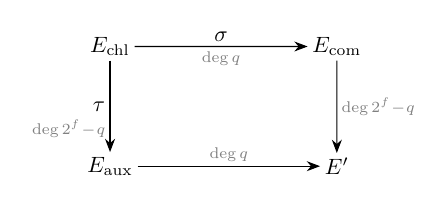
\begin{tikzpicture}[>=Stealth, every node/.style={inner sep=2pt}, scale=0.8, transform shape]
                \node (chl) at (0,1.9) {$\Echl$};
                \node (com) at (3.6,1.9) {$\Ecom$};
                \node (aux) at (0,0) {$\Eaux$};
                \node (ep)  at (3.6,0) {$E'$};
                \draw[->] (chl) -- node[above] {$\sigma$} node[below,font=\scriptsize,gray] {$\deg q$} (com);
                \draw[->] (aux) -- node[above,font=\scriptsize,gray] {$\deg q$} (ep);
                \draw[->] (chl) -- node[left] {$\tau$} node[left,yshift=-10pt,font=\scriptsize,gray] {$\deg 2^f\!-\!q$} (aux);
                \draw[->] (com) -- node[right,font=\scriptsize,gray] {$\deg 2^f\!-\!q$} (ep);
            \end{tikzpicture}
            \caption*{\small (a) dimension 2: $\tau$ is an isogeny to a new curve;
                the signer computes it and $\Eaux$ is sent}
        \end{subfigure}
        \hfill
        \begin{subfigure}[b]{0.54\textwidth}
            \centering
            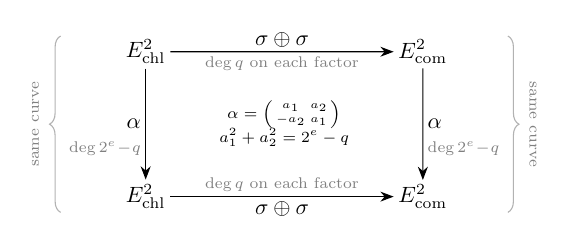
\begin{tikzpicture}[>=Stealth, every node/.style={inner sep=2pt}, scale=0.8, transform shape]
                \node (chl) at (0,2.3) {$\Echl^2$};
                \node (com) at (4.4,2.3) {$\Ecom^2$};
                \node (chl2) at (0,0) {$\Echl^2$};
                \node (com2) at (4.4,0) {$\Ecom^2$};
                \draw[->] (chl) -- node[above] {$\sigma \oplus \sigma$} node[below,font=\scriptsize,gray] {$\deg q$ on each factor} (com);
                \draw[->] (chl2) -- node[below] {$\sigma \oplus \sigma$} node[above,font=\scriptsize,gray] {$\deg q$ on each factor} (com2);
                \draw[->] (chl) -- node[left] {$\alpha$} node[left,yshift=-11pt,font=\scriptsize,gray] {$\deg 2^e\!-\!q$} (chl2);
                \draw[->] (com) -- node[right] {$\alpha$} node[right,yshift=-11pt,font=\scriptsize,gray] {$\deg 2^e\!-\!q$} (com2);
                \node[font=\scriptsize] at (2.2,1.15) {$\begin{array}{c}\alpha = \left(\begin{smallmatrix} a_1 & a_2 \\ -a_2 & a_1 \end{smallmatrix}\right)\\[2pt] a_1^2 + a_2^2 = 2^e - q\end{array}$};
                \draw[decorate,decoration={brace,amplitude=4pt},gray!60] (-1.35,-0.25) -- (-1.35,2.55);
                \node[font=\scriptsize,gray,rotate=90] at (-1.75,1.15) {same curve};
                \draw[decorate,decoration={brace,amplitude=4pt,mirror},gray!60] (5.75,-0.25) -- (5.75,2.55);
                \node[font=\scriptsize,gray,rotate=-90] at (6.15,1.15) {same curve};
            \end{tikzpicture}
            \caption*{\small (b) dimension 4: the auxiliary $\alpha$ is a pair of
                integers computed by the verifier from $q$; there is no auxiliary curve,
                so none is sent}
        \end{subfigure}
        \caption{The two ways a verifier rebuilds the response; both are Kani
            squares. (a) In dimension 2 the response $\sigma$ of degree $q$ is
            completed by an auxiliary isogeny $\tau$ of degree $2^f - q$ to a new
            curve; the signer computes $\tau$ and the signature carries $\Eaux$. (b) In
            dimension 4 the same square sits on the doubled curves and the complement
            is the endomorphism
            $\alpha = \left(\begin{smallmatrix} a_1 & a_2 \\ -a_2 & a_1 \end{smallmatrix}\right)$
            with $a_1^2 + a_2^2 = 2^e - q$, which the verifier computes from $q$; it
            acts on $\Echl^2$ and on $\Ecom^2$ alike, so each column of the square is
            one curve and there is no auxiliary curve to send. The signature carries
            $\Ecom$, $q$ and the action of $\sigma$ on the $2^r$-torsion.}
        \label{fig:kani}
    \end{figure}

    \paragraph{Which entry is dropped}
    Write the transmitted action as
    $M = \left(\begin{smallmatrix} a & b \\ c & d \end{smallmatrix}\right)$,
    so that $ad - bc \equiv kq \pmod{2^r}$. Both bases pair to roots of unity
    of exact order $2^r$, so $k$ is odd; $q$ is odd too, so $\det M$ is odd.
    Recovering the dropped entry means inverting another entry modulo $2^r$,
    which must therefore be odd, and no single entry is odd on every
    signature. The rule: if $a$ is odd, the signer drops $d$ and the verifier
    computes $d \equiv (kq + bc) \, a^{-1} \pmod{2^r}$; if $a$ is even, then
    $bc \equiv -kq$ is odd, so $b$ and $c$ are both odd, and the signer drops
    $c$, which the verifier computes as $c \equiv (ad - kq) \, b^{-1}
    \pmod{2^r}$. The verifier reads the case from the parity of $a$, so the
    rule costs no bit. The relation fixes $r$ bits of the matrix and the
    format spends them on one entry; sending all four entries and only the
    top $e - r$ bits of $q$, whose low $r$ bits the relation would then
    determine, would cost the same, so the pairings have nothing more to give.

    \paragraph{Packing the signature}
    The layout above rounds every field up to whole bytes: at level I each
    scalar takes 12 bytes for 89 bits, and $q$ takes 22 bytes for 174 bits,
    two of which are known in advance since $q \equiv 3 \pmod 4$. Writing the
    commitment curve's Montgomery coefficient as two $\lceil \log_2 p
    \rceil$-bit integers, $(q - 3)/4$ in $e - 2$ bits, the three scalars in $r$
    bits each and the two hints in 8 bits each, padded once at the end, takes
    $2 \lceil \log_2 p \rceil + (e - 2) + 3r + 16$ bits: 1107, 1690 and 2223,
    that is 139, 212 and 278 bytes at levels I, III and V, against 142, 214
    and 280 (Table~\ref{tab:params}). If each hint is a deterministic function
    of its curve, as in the round-3 specification, the verifier, which builds
    both curves, can recompute the hints instead of reading them, for 137, 210
    and 276 bytes, at the cost of searching for the bases instead of decoding
    them. The signatures measured in Section~\ref{sec:bench} use the
    byte-aligned layout; the bit-packed one changes only the encoding.

    \paragraph{Parameters for the round-3 primes}
    SQIsignHD's exponent $e$ bounds the response degree, $q < 2^e$. Every
    ideal class contains an ideal of norm at most about
    $0.90\sqrt{p}$~\cite[Lemma 12]{DLRW24}, so $2^e$ must exceed $\sqrt{p}$,
    and the paper takes ``a few bits over $\sqrt{p}$'' as sufficient on
    heuristic grounds (their Section 4.2). The library's rule $e = \lambda +
    \lceil \log_2 2\lambda \rceil$ is phrased in terms of the security
    parameter because it was set for primes with $p \approx 2^{2\lambda}$,
    where it amounts to $\log_2 \sqrt{p}$ plus 10 to 13 bits. The round-3
    level-I prime has 70 bits more than $2^{2\lambda}$, and there the same
    formula gives $2^e = 2^{136}$, below $2^{162.6}$, the bound under which
    Lemma 12 guarantees an ideal in every class: no response would exist. What
    transfers is the content of the rule, $\sqrt{p}$ plus about ten bits.

    We take $e = \lceil (\log_2 p)/2 \rceil + 11 = 174/264/346$ and, by the
    library's rule for the torsion the two half-chains need, $r = \lceil e/2
    \rceil + 2 = 89/134/175$ (Table~\ref{tab:params}). The margin of 11 bits
    lies within the 10 to 13 bits that the library's rule gives on the primes
    it was written for; SQIsignHD's own prime uses 15.3. Two checks bound it
    from below. First, the number of ideal vectors of norm below $2^e$ grows as
    $2^{2 \cdot \mathrm{margin}}$: about $2^{22}$ candidates, against one good
    norm in a few hundred, so a good $q$ exists with overwhelming probability.
    Second, Nakagawa and Onuki's conservative countermeasure for PRISM-id,
    whose response reveals an isogeny of large prime degree, is a degree of at
    least $4\lambda/3$ bits~\cite[Section 5.3]{NO25}; transferred to $e$, that
    is 170.7/256.0/341.3 against 174/264/346, cleared at every level, whereas a
    margin of 7 bits would fail it at level I.

    \paragraph{The degree}
    The signer samples vectors of the response ideal below $2^e$ and keeps the
    first whose norm $q$ is odd, congruent to 3 modulo 4, and has $2^e - q$ a
    probable prime (40 Miller--Rabin rounds). The verifier repeats the test on
    $q$ and decomposes $2^e - q$ by Cornacchia's algorithm. The sampled norms
    are odd, so one candidate in two passes the congruence; if $2^e - q$
    behaves as a random $e$-bit integer, the density of good $q$ is then $1/(e
    \ln 2)$: one candidate in 121 at level I, of which 60 reach a primality
    test. Section~\ref{sec:bench} measures the loop.

    \paragraph{What the verifier checks}
    The verifier decodes the key and the signature; recomputes the challenge;
    completes the dropped scalar by the rule above; tests $q$ for goodness and
    writes $2^e - q = a_1^2 + a_2^2$ by Cornacchia's algorithm; and builds the
    kernel of the dimension-4 isogeny on $\Ecom^2 \times \Echl^2$ from $a_1$,
    $a_2$ and the transmitted action~\cite[Lemma 4 and Section 4.4]{DLRW24}. It
    then computes the two half-chains of $\lceil e/2 \rceil$ steps from both
    ends, and accepts when the two middle codomains agree and the image of a
    point through the chain is what the transmitted action says, the two
    conditions of SQIsignHD's Section 4.5. A signature fails on any decoding
    error, on a degree that is not good, on a chain that lands on a product of
    curves where it should not, or on either condition.

    \paragraph{Whose choices}
    SQIsignHD's: the response as an ideal of good norm and the goodness test;
    the half-chains of $\lceil e/2 \rceil$ steps from both ends, with $r =
    \lceil e/2 \rceil + 2$; the action modulo $2^r$ with one scalar recovered
    from the pairing; the two acceptance conditions; and the library's
    basis-from-hint convention, kept so that its verifier checks our
    signatures unmodified. Ours: the move to the round-3 primes, $e$ and its
    margin; the round-3 commitment and $2\lambda$-bit challenge, recomputed
    rather than sent; the wire format, with two hint bytes in place of the
    library's packed bits, and its bit-packed variant; and the signer's
    sampler, which draws lattice vectors of the response ideal and rejects on
    goodness.

    \begin{table}[t]
        \centering
        \begin{threeparttable}
            \caption{Dimension-4 parameters at the round-3 primes. Level I is built
                and measured; levels III and V are derived only.}
            \label{tab:params}
            \begin{tabular}{l c c c}
                \toprule
                & NIST I & NIST III & NIST V \\
                \midrule
                $p$\tnote{a} & $3 \cdot 2^{324} - 1$ & $27 \cdot 2^{500} - 1$ & $17 \cdot 2^{664} - 1$ \\
                $\log_2 p$\tnote{a} & 325.58 & 504.75 & 668.09 \\
                $\lambda$, challenge bits\tnote{a} & 128 & 192 & 256 \\
                $e$, response bound $q < 2^e$\tnote{b} & 174 & 264 & 346 \\
                $r = \lceil e/2 \rceil + 2$, transmitted torsion bits\tnote{c} & 89 & 134 & 175 \\
                half-chain steps $\lceil e/2 \rceil$\tnote{c} & 87 & 132 & 173 \\
                \addlinespace
                public key, bytes, predicted\tnote{d} & 84 & 130 & 170 \\
                signature, bytes, predicted\tnote{d} & 142 & 214 & 280 \\
                signature, bytes, bit-packed\tnote{e} & 139 & 212 & 278 \\
                public key, bytes, measured & 84 & {\color{red}not built} & {\color{red}not built} \\
                signature, bytes, measured & 142 & {\color{red}not built} & {\color{red}not built} \\
                round-3 standard signature, bytes\tnote{a} & 200 & 306 & 406 \\
                \bottomrule
            \end{tabular}
            \begin{tablenotes}\footnotesize
                \item[a] The {\SQIsign} round-3 specification~\cite{AAA+26}.
                \item[b] Ours: $e = \lceil (\log_2 p)/2 \rceil + 11$ (Section~\ref{sec:dim4}).
                \item[c] SQIsignHD's rule for the torsion the half-chains need~\cite[Section 4.3]{DLRW24}.
                \item[d] Field-by-field sums of the byte-aligned wire format (Section~\ref{sec:dim4}).
                \item[e] $2 \lceil \log_2 p \rceil + (e - 2) + 3r + 16$ bits, padded once (Section~\ref{sec:dim4}); 137 / 210 / 276 without the hints.
            \end{tablenotes}
        \end{threeparttable}
    \end{table}

    %% ============================================================
    \section{Benchmarks}
    \label{sec:bench}
    %% ============================================================

    \paragraph{Method}
    All measurements come from one session on one machine, an AMD EPYC 7B13
    guest (16 vCPUs, 63~GiB; the cycle counter at 3049.994~MHz), on
    2026-11-02. One binary measures the Rust code, compiled by \texttt{rustc}
    1.99.1 in release mode with fat link-time optimization and no target-CPU
    flag; the code chooses its assembly field kernels at run time from CPUID.
    Each operation is timed with \texttt{rdtsc} and the wall clock around the
    call, on one pinned core, in four rounds that visit every block in turn;
    the tables report medians over 52 runs for key generation and signing in
    dimension 2, 200 for verification, and, for the compact format, 52 for key
    generation, 100 for signing and 200 for each verifier. Verification is
    measured from bytes: decode the key, decode the signature, verify.

    \paragraph{Sizes}
    Table~\ref{tab:sizes} lists the sizes on the wire. At level I the compact
    key and signature take 226 bytes and 223 bit-packed, against
    283 for the specification's format: a saving of 29\,\% on the signature,
    or 30.5\,\% bit-packed. The compressed dimension-2 format, with a 174-byte
    signature, sits between them.

    \begin{table}[t]
        \centering
        \begin{threeparttable}
            \caption{Public key + signature = total, in bytes, at the round-3
                primes. Compact formats are level I only.}
            \label{tab:sizes}
            \footnotesize
            \setlength{\tabcolsep}{3.5pt}
            \begin{tabular}{l c c c}
                \toprule
                format & NIST I & NIST III & NIST V \\
                \midrule
                standard (specification) & $83 + 200 = 283$ & $129 + 306 = 435$ & $169 + 406 = 575$ \\
                compressed (this crate)\tnote{a} & $83 + 174 = 257$ & $129 + 267 = 396$ & $169 + 352 = 521$ \\
                compact, dim.\ 4 (this crate) & $84 + 142 = 226$ & {\color{red}not built} & {\color{red}not built} \\
                compact, dim.\ 4, bit-packed\tnote{b} & $84 + 139 = 223$ & $130 + 212 = 342$ & $170 + 278 = 448$ \\
                \bottomrule
            \end{tabular}
            \begin{tablenotes}\footnotesize
                \item[a] The compressed format's current layout. The session of Section~\ref{sec:bench} measured the earlier layout of 176 / 269 / 353 bytes.
                \item[b] Predicted from the layout of Section~\ref{sec:dim4}, not observed in the session; levels III and V use the predicted public keys of Table~\ref{tab:params}.
            \end{tablenotes}
        \end{threeparttable}
    \end{table}

    \paragraph{Cycles}
    Table~\ref{tab:cycles} gives the session in megacycles. At level I the
    dimension-4 verifier costs 6.4 times the dimension-2 verifier of the same
    crate with four kernel points and 4.6 times with two, and dimension-4
    signing costs 2.9 times dimension-2 signing, because the good degree is
    found by rejection (Table~\ref{tab:loop}). Key generation is the same in
    both formats up to the basis convention (40.8 against 38.5 megacycles);
    the compressed format's recovery adds 16\,\% to a verification.

    \begin{table}[t]
        \centering
        \caption{Megacycles at the round-3 primes, medians of the session. The
            last column is the dimension-4 verifier over the dimension-2 verifier of
            the same code.}
        \label{tab:cycles}
        \begin{tabular}{l c r r r r}
            \toprule
            implementation & level & keygen & sign & verify & $\times$ dim.\ 2 \\
            \midrule
            Rust, dimension 2 & I   & 38.5  & 112.5 & 13.3 & \\
            Rust, dimension 2 & III & 142.2 & 392.9 & 33.7 & \\
            Rust, dimension 2 & V   & 257.0 & 787.5 & 80.7 & \\
            Rust, dimension 2, compressed verify & I & & & 15.4 & \\
            Rust, dimension 4 (compact) & I & 40.8 & 329.0 & 85.4 & 6.4 \\
            Rust, dim.\ 4, two points, checked & I & & & 60.6 & 4.6 \\
            Rust, dim.\ 4, two points, unchecked & I & & & 59.6 & 4.5 \\
            \bottomrule
        \end{tabular}
    \end{table}

    \begin{figure}[t]
        \centering
        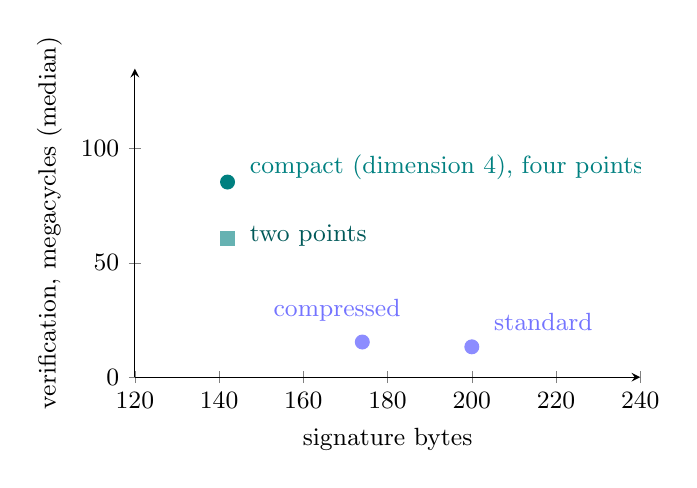
\begin{tikzpicture}
            \begin{axis}[
                width=8cm, height=5.5cm,
                xmin=120, xmax=240, ymin=0, ymax=135,
                xlabel={signature bytes},
                ylabel={verification, megacycles (median)},
                axis lines=left,
                xtick={120,140,...,240}, ytick={0,50,100},
                tick label style={font=\small}, label style={font=\small},
                every node near coord/.append style={font=\small},
                ]
                \addplot[only marks, mark=*, mark size=2.5pt, color=teal] coordinates {(142,85.4)};
                \addplot[only marks, mark=square*, mark size=2.5pt, color=teal!60] coordinates {(142,60.6)};
                \addplot[only marks, mark=*, mark size=2.5pt, color=blue!45] coordinates {(174,15.4) (200,13.3)};
                \node[teal, anchor=west, font=\small] at (axis cs:145,92) {compact (dimension 4), four points};
                \node[teal!70!black, anchor=west, font=\small] at (axis cs:145,62) {two points};
                \node[blue!55, anchor=south, font=\small] at (axis cs:168,20) {compressed};
                \node[blue!55, anchor=south west, font=\small] at (axis cs:203,16) {standard};
            \end{axis}
        \end{tikzpicture}
        \caption{The trade at level I on the round-3 prime: signature bytes
            against verification cost for the three formats of one crate, the compact one with four and with two kernel points, from the
            session of Table~\ref{tab:cycles}. The compressed format is placed at its
            current size of 174 bytes; its verification cost was measured with the
            earlier 176-byte layout.}
        \label{fig:trade}
    \end{figure}

    \paragraph{Milliseconds}
    Table~\ref{tab:ms} gives wall-clock times at level I on two machines.
    Neither is what a deployment runs; the ratio between the rows is the
    number to carry.

    \begin{table}[t]
        \centering
        \caption{Milliseconds at level I on the round-3 prime, medians, on the EPYC 7B13 guest of Section~\ref{sec:bench} (megacycles over its counter rate of 3049.994\,MHz) and on an M4 Pro. The M4 Pro column is
            pending a run on that machine.}
        \label{tab:ms}
        \small
        \setlength{\tabcolsep}{4pt}
        \begin{tabular}{l l r r}
            \toprule
            format & operation & EPYC (ms) & M4 Pro (ms) \\
            \midrule
            dimension 2 (standard) & key generation & 12.6 & {\color{red}pending} \\
            & signing & 36.9 & {\color{red}pending} \\
            & verification & 4.4 & {\color{red}pending} \\
            & verification, compressed & 5.0 & {\color{red}pending} \\
            \addlinespace
            dimension 4 (compact) & key generation & 13.4 & {\color{red}pending} \\
            & signing & 107.9 & {\color{red}pending} \\
            & verification & 28.0 & {\color{red}pending} \\
            \bottomrule
        \end{tabular}
    \end{table}

    \paragraph{The rejection loop}
    Table~\ref{tab:loop} compares the compact signer's search for a good
    degree over the session's signatures with the expectation of
    Section~\ref{sec:dim4}. A candidate costs one norm computation; one in two
    reaches a Miller--Rabin test on an $e$-bit number, and composites fail at
    the first round. This loop accounts for the spread of signing times: the
    median signature needs 79.5 samples, the mean 111.6, and the range is 2 to
    523.

    \begin{table}[t]
        \centering
        \caption{The compact signer's good-degree loop at level I: measured over
            the session's signatures against the density $1/(e \ln 2)$ for odd $q$
            (and the figure for a candidate of random parity, which the sampler does
            not produce).}
        \label{tab:loop}
        \begin{tabular}{l r r}
            \toprule
            & measured & expected \\
            \midrule
            signatures measured & 100 & \\
            response samples per signature, mean & 111.6 & 121 \\
            the same if $q$ had random parity & {\color{red}???} & 241 \\
            response samples per signature, median (min, max) & 79.5 (2, 523) & \\
            primality tests per signature, mean & 54.8 & 60 \\
            signing, Mcycles, median (min, max) & 329.0 (48.8, 1900.9) & \\
            signing, dimension 2, Mcycles, median & 112.5 & \\
            \bottomrule
        \end{tabular}
    \end{table}

    \paragraph{Memory}
    At its peak, one compact verification at level I allocates 1674~KiB
    (1.64~MiB) of heap, measured with a counting allocator around the call in a session of 2026-09-26;
    the dimension-2 verifier allocates nothing.

    %% ============================================================
    \section{Strong unforgeability and ECLIPSE}
    \label{sec:suf}
    %% ============================================================

    A signature scheme is strongly unforgeable when no one can produce a
    second valid signature on a message already signed. The {\SQIsign} family
    is not: in the dimension-2 format the auxiliary isogeny can be replaced by
    another of the same degree, giving a second signature valid under the same
    key, as the round-3 specification states in its Section
    8.4.2~\cite{AAA+26}; the mechanism is written out in~\cite{Ray26a}.
    Dimension 4 removes the auxiliary curve from the wire but not the property:
    another isogeny of the same degree from the same commitment curve, with
    its own action on the torsion, is still a valid second signature. This is
    a property of the scheme, not a finding of this paper.

    A construction that is strongly unforgeable by design exists. Next to
    their salted scheme, the PRISM authors describe a variant whose signature
    is a single isogeny of prime degree $2^{2e-1} - s^2$ from the public-key
    curve, and state that the EUF-CMA proof of the salted scheme applies to a
    salted version of it~\cite[Section 5 and Remark 11]{BBC+26}; we call that
    variant strong-PRISM. Our instantiation of it on the round-3 primes,
    ECLIPSE\footnote{ECLIPSE stands for Encoding-Canonical Large-prime Isogeny
        Signature Extension. The underlying construction, which we call
        strong-PRISM, is Section 5 of~\cite{BBC+26} with the salt of Section 6 as
        suggested in Remark 11; the authors did not name it.}, is the subject
    of a forthcoming paper.

    Dimension 4 buys strong-PRISM nothing. A PRISM signature carries no
    auxiliary curve in any dimension, so there is nothing to remove; a
    dimension-4 instantiation would have the same layout within a few bytes,
    and its hash target, a prime $q$ with $2^a - q$ prime and congruent to 1
    modulo 4, needs two primality conditions at once, a far sparser target
    than the single prime of the dimension-2 variant. A feasibility study for
    prism-rs~\cite{Ray26b} measured both and declined the dimension-4 route.

    %% ============================================================
    \section{Conclusion}
    \label{sec:conc}
    %% ============================================================

    SQIsignHD's dimension-4 response carries over to the round-3 {\SQIsign}
    primes once its response bound is restated in terms of $\sqrt{p}$ rather
    than the security parameter, and it keeps its defining advantage there:
    with no auxiliary curve to send, a level-I signature takes 142 bytes as
    built and 139 bit-packed, against 200 for the specification's format, and
    key and signature together take 226 bytes, or 223, the smallest level-I
    combination we are aware of at parameters that stand after the 2026
    attack.

    The verifier pays for it. In the same code, a dimension-4 verification
    costs 6.4 times a dimension-2 one at level I (85.4 against 13.3
    megacycles), 4.6 times with the two-point verifier below, and needs about
    1.6~MiB of heap where the dimension-2 verifier needs none; signing costs
    2.9 times as much, because of the search for a
    good degree. The compact format therefore suits settings where bandwidth
    or storage dominates and a verification of a few tens of milliseconds is
    acceptable; the specification's dimension-2 format remains the better
    general-purpose choice. Neither format makes {\SQIsign} strongly
    unforgeable; that requires a different construction, such as the PRISM
    variant of Section~\ref{sec:suf}.

    \paragraph{Two-point verification}
    The verifier's chain respects an automorphism of order 4, as MIKE's does.
    On $E^2$ the automorphism $J = \left(\begin{smallmatrix} 0 & 1 \\ -1 & 0
    \end{smallmatrix}\right)$ satisfies $J^2 = -1$ and $\alpha = a_1 + a_2 J$,
    so both $\alpha$ and $\sigma \oplus \sigma$ commute with $J$ acting on
    $\Echl^2$ and $\Ecom^2$ alike (Appendix~\ref{app:symmetry}). In every test
    we ran, the resulting automorphism of the fourfold acts on the theta
    coordinates our verifier uses as one fixed permutation of the sixteen
    coordinates, at every step of both half-chains, and maps two of the four
    kernel generators onto the other two. We prove that both facts hold at
    every step from the gluing on, for every input, honest or not, for the
    algorithm the verifier implements (Theorem~\ref{thm:base}); {\color{red}that
        our implementation computes that algorithm's theta structures is checked
        only in part (Remark~\ref{rem:conformance})}. A verifier can therefore
    double and push only two kernel points along each half-chain and obtain
    the other two by permuting coordinates. We have implemented this variant
    as an option of our Rust port; it checks the condition at the gluing on
    each signature and falls back to four points otherwise. In the session of
    Section~\ref{sec:bench}, two-point verification with the check costs 60.6
    megacycles at level I against 85.4 for the four-point verifier, 0.71 of
    it, and 59.6 without the check, 0.70. In the port's tests, the two-point
    and the four-point verifier return the same verdict and the same
    rejection reason on the five level-I vectors and on 70 distinct tampered
    inputs, and the same codomain null point at each of the 844 plain steps
    of both half-chains over the five vectors, in both two-point modes.

    \paragraph{Limitations}
    There is only one implementation, and no independent round-3 dimension-4
    signer to compare against. The SQIsignHD authors' verifier,
    re-parameterized to our prime and otherwise unmodified, accepts our
    signatures and rejects tampered ones~\cite{DLRW25}, which shows that it
    agrees with our verifier on our signer's output and nothing more. Levels
    III and V are derived in Table~\ref{tab:params} but not built, and the
    bit-packed layout of Section~\ref{sec:dim4} is specified and sized but not
    implemented. Constant-time execution was not attempted for the
    dimension-4 signer or verifier: the verifier's integer arithmetic on the
    degree is variable-time on public data, and {\SQIsign} signing is
    variable-time by design in the reference as well. The security argument is
    SQIsignHD's with our parameters substituted and has not been re-examined;
    the existence of a good degree in every class is a heuristic in their
    paper and remains one here. The two-point verifier is tested at level I
    only, on five vectors and their tampered variants, and is not the
    default; {\color{red}its
        correctness for every input rests on the conformance of the implementation
        to the algorithm of Theorem~\ref{thm:base}, which is checked only in part
        (Remark~\ref{rem:conformance})}. The format is experimental and not for
    production.

    \paragraph{Outlook}
    Each limitation above is also a next step. Beyond them, faster dimension-4
    arithmetic would narrow the gap in verification cost, which decides
    whether the 58 bytes saved at level I are worth having, and there is
    reason to expect room. MIKE's chain costs about 0.07 megacycles per step
    at level I, against about 0.49 for our four-point verifier and 0.35 for
    the two-point one (85.4 and 60.6 megacycles over $2 \cdot 87$ steps). The
    comparison is loose, since MIKE works over $\mathbb{F}_p$ on a different
    processor and our verifier also evaluates a point for its image check,
    but it suggests that much of our 6.4-fold penalty lies in the
    implementation rather than in the dimension (measured below: 1.18 of the
    counted floor at our own operation count). MIKE's computation of each
    codomain from two points and its faster doubling on the quotient by the
    automorphism~\cite[Appendix E.2]{BDD+26} would save more than our
    two-point verifier, and its observation that additions, not
    multiplications, are a significant share of the cost of dimension-4 theta
    arithmetic~\cite[Section 6]{BDD+26} points toward field representations
    and vectorization tuned to the Hadamard transform.

    In our two-point verifier the plain dimension-4 steps are 67.1 percent of
    the cost (point pushes 44.9 percent, codomain computations 22.2 percent),
    the setup before the chain 19.6 percent, the dimension-2 gluing chain 0.9
    percent, the image check 6.5 percent and the gluing 6.0 percent, measured
    in the session of Section~\ref{sec:bench} (basis generation 7.48
    megacycles, Cornacchia and kernel setup 4.23, dimension-2 steps 0.52,
    gluing 3.60, point pushes 26.88, codomain computations 13.28, image check
    3.87; the whole call 60.37); the codomain computations, 33.1 percent of
    the plain steps, are the part a codomain-from-two-points step would
    address.

    The two-point verifier's operation count, taken with counters in the
    field arithmetic at the session's commit, is 132\,921 multiplications,
    91\,426 squarings, 435\,363 additions, 54 inversions and 11 square roots
    in $\mathbb{F}_{p^2}$ per verification, 51.0 megacycles at the session's
    per-operation costs; at the reference count of our floor table, which
    takes a hand count of the SQIsignHD library's code where that count is
    below ours and our own count elsewhere, the same costs give 50.8.
    Measured in the same session, the verifier runs at 1.18 of the former
    floor and 1.19 of the latter, 9.6 megacycles above the latter, 5.8 of
    them in the two plain-step phases (1.15 for the point pushes, 1.21 for
    the codomains; 1.12 for the basis, 1.16 for the setup, 1.35 for the
    gluing, 1.16 for the image check). What remains is the sixteen-coordinate
    arithmetic of the plain steps on general points: their operation count
    is the library's, and the gap sits inside the Hadamard transform and the
    squaring kernels.

    Three years separate the break of SIDH from a two-dimensional {\SQIsign} in
    a NIST round, and one more separates that from primes moved by a new
    attack on the isogeny-path problem. Every construction in this paper is
    young, ours included, and the numbers describe code as it stood in
    November 2026, not a settled design; that is the reason for caution in
    using any of it.


    \bibliographystyle{alpha}
    \bibliography{Dim4SQI}

    \appendix

    \section{The order-4 symmetry of the verifier's chain}
    \label{app:symmetry}

    This appendix proves that the verifier's chain respects an automorphism of
    order 4 and that, for the algorithm the verifier implements, the
    automorphism acts on the theta coordinates of every fourfold from the
    gluing on as one fixed permutation (Theorem~\ref{thm:base}). This is what
    lets the two-point verifier of Section~\ref{sec:conc} apply MIKE's saving
    of two kernel points out of four~\cite[Appendix E.2]{BDD+26} to the
    verifier of Section~\ref{sec:dim4}. Section~\ref{app:remains} separates
    what is established about our implementation from what remains unproven.

    \paragraph{Notation}
    Throughout, $E$ denotes a supersingular elliptic curve over
    $\mathbb{F}_{p^2}$ and $E^2 = E \times E$. Homomorphisms between squares of
    curves are written as $2 \times 2$ matrices whose entries are homomorphisms
    between the curves, acting on column vectors:
    \[
    \begin{pmatrix} u & v \\ w & z \end{pmatrix}
    \begin{pmatrix} P \\ Q \end{pmatrix}
    =
    \begin{pmatrix} u(P) + v(Q) \\ w(P) + z(Q) \end{pmatrix}.
    \]
    An integer $n$ stands for the multiplication map $[n]$. For a homomorphism
    $\psi$ we write $\widehat{\psi}$ for its dual. With respect to the product
    polarizations, the dual of a matrix is the transpose of the matrix of
    duals; in particular the dual of an integer matrix is its transpose. We
    write $\Echl$ for the challenge curve, $\Ecom$ for the commitment curve,
    $\sigma \colon \Echl \to \Ecom$ for the response, of odd degree $q$, and
    $a_1, a_2$ for integers with $a_1^2 + a_2^2 = 2^e - q$, as in
    Section~\ref{sec:dim4}. Finally
    \[
    A_1 = \Echl^2, \qquad A_2 = \Ecom^2, \qquad A = A_1 \times A_2,
    \]
    so that $A$ is the abelian fourfold on which the verifier's chain starts.

    \subsection{The automorphism \texorpdfstring{$J$}{J} of \texorpdfstring{$E^2$}{E\^{}2}}

    \begin{definition}
        On any square $E^2$, let
        \[
        J = \begin{pmatrix} 0 & 1 \\ -1 & 0 \end{pmatrix},
        \qquad\text{that is,}\qquad
        J(P, Q) = (Q, -P),
        \]
        and on $A = A_1 \times A_2$ let $D = \operatorname{diag}(J, J)$ be $J$
        acting on each square separately.
    \end{definition}

    \begin{lemma}
        \label{lem:J}
        \leavevmode
        \begin{enumerate}[label=(\roman*)]
            \item $J^2 = -1$, so $J$ has order 4.
            \item The endomorphism
            $\alpha = \left(\begin{smallmatrix} a_1 & a_2 \\ -a_2 & a_1
            \end{smallmatrix}\right)$ of Figure~\ref{fig:kani} equals
            $a_1 + a_2 J$, and its dual is
            $\widehat{\alpha} = \alpha^{\mathsf{T}} = a_1 - a_2 J$.
            \item $\widehat{\alpha}\,\alpha = \alpha\,\widehat{\alpha} = a_1^2 + a_2^2
            = 2^e - q$.
            \item $\widehat{J} = J^{\mathsf{T}} = -J = J^{-1}$, so $J$ preserves the
            product polarization of $E^2$: it is an automorphism of $E^2$ as a
            principally polarized abelian surface.
        \end{enumerate}
    \end{lemma}

    \begin{proof}
        (i) $J^2(P, Q) = J(Q, -P) = (-P, -Q)$. (ii) We have
        \[
        (a_1 + a_2 J)(P, Q) = \bigl([a_1]P + [a_2]Q, \; -[a_2]P + [a_1]Q\bigr),
        \]
        which is $\alpha(P, Q)$; the dual
        of an integer matrix is its transpose, and $J^{\mathsf{T}} = -J$. (iii)
        $(a_1 + a_2 J)(a_1 - a_2 J) = a_1^2 - a_2^2 J^2 = a_1^2 + a_2^2$, since
        $J$ commutes with integers. (iv) $J^{\mathsf{T}} J = 1$ by direct
        computation, and an automorphism $\gamma$ preserves the polarization
        exactly when $\widehat{\gamma}\gamma = 1$.
    \end{proof}

    \subsection{The verifier's isogeny commutes with \texorpdfstring{$D$}{D}}
    \label{app:kani}

    Write $\Sigma = \operatorname{diag}(\sigma, \sigma) \colon A_1 \to A_2$, the
    map $\sigma \oplus \sigma$ of Figure~\ref{fig:kani}, so that
    $\widehat{\Sigma} = \operatorname{diag}(\widehat{\sigma},
    \widehat{\sigma})$. Consider the Kani endomorphism~\cite[Section 4]{DLRW24}
    \[
    F = \begin{pmatrix} \alpha & \widehat{\Sigma} \\
        -\Sigma & \widehat{\alpha} \end{pmatrix}
    \colon A_1 \times A_2 \longrightarrow A_1 \times A_2,
    \qquad
    F(x_1, x_2) = \bigl(\alpha(x_1) + \widehat{\Sigma}(x_2), \;
    -\Sigma(x_1) + \widehat{\alpha}(x_2)\bigr),
    \]
    where the $\alpha$ in the top-left corner acts on $A_1$ and the
    $\widehat{\alpha}$ in the bottom-right corner on $A_2$. Its dual is
    \[
    \widehat{F} = \begin{pmatrix} \widehat{\alpha} & -\widehat{\Sigma} \\
        \Sigma & \alpha \end{pmatrix}.
    \]
    The verifier's dimension-4 isogeny is this endomorphism with the roles of
    the two curves exchanged: $(\Echl, \Ecom, \sigma)$ replaced by $(\Ecom,
    \Echl, \widehat\sigma)$, so that it acts on $\Ecom^2 \times \Echl^2$
    (Lemma~\ref{lem:kanimat} gives it explicitly). Nothing below depends on
    which curve is which, so every statement about $F$ and $\widehat F$ applies
    to it.

    \begin{lemma}
        \label{lem:kani}
        $\widehat{F} F = F \widehat{F} = 2^e$. Hence $F$ is an isogeny of degree
        $2^{4e}$, and $\ker F = \widehat{F}\bigl(A[2^e]\bigr)$.
    \end{lemma}

    \begin{proof}
        Every entry of $F$ and $\widehat{F}$ is an integer matrix or a
        componentwise map $\operatorname{diag}(\psi, \psi)$, and these commute with
        each other: for an integer matrix $M$ and any homomorphism $\psi$ of
        curves, $\operatorname{diag}(\psi, \psi) M = M \operatorname{diag}(\psi,
        \psi)$, because $\psi$ is a group homomorphism. The diagonal blocks of
        $\widehat{F} F$ are $\widehat{\alpha}\alpha + \widehat{\Sigma}\Sigma =
        (2^e - q) + q = 2^e$ and $\Sigma\widehat{\Sigma} + \alpha\widehat{\alpha}
        = 2^e$, by Lemma~\ref{lem:J}(iii) and $\widehat{\sigma}\sigma =
        \sigma\widehat{\sigma} = q$; the off-diagonal blocks are
        $\widehat{\alpha}\widehat{\Sigma} - \widehat{\Sigma}\widehat{\alpha} = 0$
        and $\Sigma\alpha - \alpha\Sigma = 0$. The same holds for
        $F\widehat{F}$. Then $(\deg F)^2 = \deg [2^e] = 2^{8e}$ on a fourfold, so
        $\deg F = 2^{4e}$. Finally $\widehat{F}(A[2^e]) \subseteq \ker F$ because
        $F\widehat{F} = 2^e$, and both groups have $2^{4e}$ elements, since
        $\ker \widehat{F} \subseteq A[2^e]$ has $2^{4e}$ elements and
        $|A[2^e]| = 2^{8e}$.
    \end{proof}

    \begin{proposition}
        \label{prop:commute}
        $F \circ D = D \circ F$. In particular $\ker F$ is stable under $D$.
    \end{proposition}

    \begin{proof}
        Since $D = \operatorname{diag}(J, J)$, the identity $FD = DF$ holds block
        by block exactly when each block of $F$ commutes with $J$. The blocks
        $\alpha$ and $\widehat{\alpha}$ are polynomials in $J$
        (Lemma~\ref{lem:J}(ii)), and $\Sigma$, $\widehat{\Sigma}$ are componentwise
        maps, which commute with every integer matrix (proof of
        Lemma~\ref{lem:kani}). Explicitly, $J\Sigma(P, Q) = J(\sigma P, \sigma Q)
        = (\sigma Q, -\sigma P) = \Sigma(Q, -P) = \Sigma J(P, Q)$. If $F(x) = 0$
        then $F(D x) = D F(x) = 0$. The blocks of $\widehat F$ are of the same
        kinds, so $\widehat F D = D \widehat F$ as well.
    \end{proof}

    \subsection{Consequences along the chain}

    The verifier computes $F$ as a chain of $e$ isogenies of degree 2. Write
    $K = \ker F$ and, for $0 \le k \le e$, let $F_k \colon A \to A_k =
    A / [2^{e-k}]K$ be the partial chain after $k$ steps, so that $F_e = F$ up
    to isomorphism. The two half-chains that meet in the middle are partial
    chains of this kind, one read from each end.

    \begin{proposition}
        \label{prop:descent}
        For every $k$, there is an automorphism $D_k$ of $A_k$ with
        $D_k \circ F_k = F_k \circ D$. It satisfies $D_k^2 = -1$ and
        $\widehat{D_k} = -D_k$, and it preserves the principal polarization of
        $A_k$.
    \end{proposition}

    \begin{proof}
        $D$ is a group automorphism with $D(K) = K$
        (Proposition~\ref{prop:commute}), hence $D([2^{e-k}]K) = [2^{e-k}]K$, so
        $F_k \circ D$ vanishes on $\ker F_k$ and factors as $D_k \circ F_k$; $D_k$
        is an automorphism because $D$ is. The identities $D_k^2 = -1$ and
        $\widehat{D_k} = -D_k$ follow from $D^2 = -1$ and $\widehat{D} = -D$
        (Lemma~\ref{lem:J}) by uniqueness of the factorization. The principal
        polarization of $A_k$ is the one induced from $2^k$ times that of $A$
        through the isotropic kernel $\ker F_k$; $D$ preserves both, so $D_k$
        preserves the induced one.
    \end{proof}

    \begin{remark}[The module viewpoint]
        \label{rem:module}
        The varieties here are maximal: each curve has $(p+1)^2$ points over
        $\mathbb{F}_{p^2}$. By the anti-equivalence $A \mapsto M_A =
        \operatorname{Hom}(A, E_0)$ of~\cite[Theorem 2.5]{PRS26}, under which
        principal polarizations correspond to unimodular Hermitian forms $H_A$ and
        isogenies to module monomorphisms~\cite[Table 1]{PRS26}, the automorphism
        $D$ corresponds to $f \mapsto f \circ D$ on $M_A$, which preserves $H_A$
        by Lemma~\ref{lem:J}(iv) and squares to $-1$. The partial chain $F_k$
        corresponds to the inclusion $\psi_k \colon M_{A_k} \hookrightarrow M_A$,
        $f \mapsto f \circ F_k$, whose image consists of the morphisms vanishing on
        $\ker F_k$. Since $D(\ker F_k) = \ker F_k$, that image is stable under
        $f \mapsto f \circ D$, and $f \circ D_k \circ F_k = f \circ F_k \circ D$
        shows that $D_k$ corresponds to the restriction of $f \mapsto f \circ D$
        to it. This is Proposition~\ref{prop:descent} in module form: $D$
        descends along the chain exactly because each partial kernel, equivalently
        each image submodule, is $D$-stable.
    \end{remark}

    \begin{proposition}
        \label{prop:weil}
        Every $A_k$ is of Weil type in the sense of~\cite[Definition 4.1]{BDD+26}:
        $D_k$ embeds $\mathbb{Z}[i]$ in $\operatorname{End}(A_k)$, with
        $i \mapsto D_k$, and acts on the tangent space at the origin with
        eigenvalues $i, i, -i, -i$.
    \end{proposition}

    \begin{proof}
        On the tangent space of $E^2$ the differential of $J$ is the matrix
        $\left(\begin{smallmatrix} 0 & 1 \\ -1 & 0 \end{smallmatrix}\right)$,
        whose eigenvalues are $i$ and $-i$; these lie in $\mathbb{F}_{p^2}$ because
        $p \equiv 3 \pmod 4$. Hence $D = \operatorname{diag}(J, J)$ has eigenvalues
        $i, i, -i, -i$ on the tangent space of $A$. Isogenies of degree a power of
        2 are separable in odd characteristic, so the differential of $F_k$ is an
        isomorphism, and it intertwines $D$ with $D_k$
        (Proposition~\ref{prop:descent}); the eigenvalues are therefore the same.
        This is the argument of~\cite[proof of Proposition G.1]{BDD+26}.
    \end{proof}

    \begin{proposition}
        \label{prop:forged}
        For any matrix the verifier receives, honest or not, the kernel it builds
        is stable under $D$. Whenever that kernel defines a chain, that is, when it
        is maximal isotropic and the computation succeeds, the conclusions of
        Propositions~\ref{prop:descent} and~\ref{prop:weil} hold for that chain.
    \end{proposition}

    \begin{proof}
        The verifier builds its kernel from the transmitted action rather than
        from $\sigma$: the transmitted matrix defines a map $\sigma'$ on the
        $2^r$-torsion (the map $\tau$ of Section~\ref{app:conjecture}, with the
        curves exchanged as in Section~\ref{app:kani}), and the verifier uses $\Sigma' = \operatorname{diag}(\sigma',
        \sigma')$ in place of $\Sigma$. Like $\Sigma$, the map $\Sigma'$ acts
        componentwise, so it commutes with $J$, and the kernel generators
        $(\widehat{\alpha}(x), \Sigma'(x))$ satisfy $D(\widehat{\alpha}(x),
        \Sigma'(x)) = (\widehat{\alpha}(Jx), \Sigma'(Jx))$, which is again of that
        form. The proofs of Propositions~\ref{prop:descent} and~\ref{prop:weil} use
        only that the kernel is $D$-stable and that the chain has 2-power degree.
    \end{proof}

    \subsection{The kernel as a module over \texorpdfstring{$\mathbb{Z}[i]$}{Z[i]}}

    Let $R_e = (\mathbb{Z}/2^e)[i]$, acting on $2^e$-torsion with $i$ acting as
    $J$ (or $D$).

    \begin{lemma}
        \label{lem:free}
        $E^2[2^e]$ is a free $R_e$-module of rank 2, and so is $\ker F$.
    \end{lemma}

    \begin{proof}
        Let $(S, T)$ be a basis of $E[2^e]$. Since $J(S, 0) = (0, -S)$ and
        $J(T, 0) = (0, -T)$, the four points
        $(S, 0), (T, 0), (0, S), (0, T)$, which form a $\mathbb{Z}/2^e$-basis of
        $E^2[2^e]$, are $(S, 0)$, $(T, 0)$, $-J(S, 0)$ and $-J(T, 0)$; so $(S, 0)$ and $(T, 0)$ form an $R_e$-basis. For the kernel,
        consider
        \[
        \iota \colon A_1[2^e] \to A, \qquad
        \iota(x) = \widehat{F}(x, 0) = \bigl(\widehat{\alpha}(x), \Sigma(x)\bigr).
        \]
        Its image lies in $\ker F$ by
        Lemma~\ref{lem:kani}. It is injective, because $\widehat{\alpha}$ has odd
        degree $(2^e - q)^2$ and is therefore injective on 2-power torsion. Its
        domain has $2^{4e}$ elements, as does $\ker F$, so $\iota$ is a bijection
        onto $\ker F$. Finally $\iota$ commutes with $J$, so it is $R_e$-linear, and
        $\ker F \cong A_1[2^e] = \Echl^2[2^e]$ is free of rank 2.
    \end{proof}

    MIKE uses the corresponding statement about its own kernel~\cite[proof of
    Corollary G.1]{BDD+26} to show that the pairing $e_{1+i}$ is alternate on
    its fourfolds, which in turn is what makes its adapted theta coordinates
    exist. On the starting fourfold $A$ the analogous pairing is alternate.

    \begin{lemma}
        \label{lem:alternate}
        The Weil--Cartier pairing $e_{1+D}$ on $A[1 + D]$ is alternate.
    \end{lemma}

    \begin{proof}
        It suffices to treat one square $E^2$, since $A$ is a product of two
        and the pairings multiply. If $(1 + J)(P, Q) = (P + Q, Q - P) = 0$, then
        $P = -Q$ and $2P = 0$, so $\ker(1 + J) = \{(u, u) : u \in E[2]\}$. With
        the formula of~\cite[proof of Corollary G.1]{BDD+26},
        $e_{1+J}(x, x) = e_2(J x_0, x_0)$ for any $x_0$ with $(1 + J) x_0 = x$.
        For $x = (u, u)$ take $x_0 = (0, u)$, since $(1 + J)(0, u) = (0, u) +
        (u, 0) = (u, u)$. Then $e_2(J x_0, x_0) = e_2\bigl((u, 0), (0, u)\bigr) =
        e_2(u, 0)\, e_2(0, u) = 1$.
    \end{proof}

    \subsection{The verifier's theta coordinates}
    \label{app:coords}

    This subsection proves how $D$ acts in level-2 theta coordinates once it
    acts correctly on the basis inducing them; Section~\ref{app:conjecture}
    proves that it does, on the theta structures of the verifier's algorithm.
    Throughout, $\pi$ is the permutation of $\{0, \ldots, 15\}$ that exchanges
    bits 0 and 2 and bits 1 and 3 of the index $a = i_0 + 2 i_1 + 4 i_2 + 8
    i_3$; it is an involution. We identify $a$ with its multi-index $\mathbf i =
    (i_0, i_1, i_2, i_3) \in \{0, 1\}^4$, write $\theta_{\mathbf v}$ for
    $\theta_{\mathbf v \bmod 2}$ when $\mathbf v$ is an integer vector, and
    $\langle \mathbf i \mid \mathbf j \rangle = \sum_l i_l j_l$.

    \paragraph{Theta structures and bases}
    Let $A'$ be a principally polarized abelian fourfold over an algebraically
    closed field $\Bbbk$ of odd characteristic (the varieties of the chain are
    defined over $\mathbb F_{p^2}$, and we work over its algebraic closure, as
    does~\cite[Section 2]{Dar24}), let $\mathcal L = \mathcal L_0^2$ with $\mathcal L_0$ a
    symmetric line bundle representing the principal polarization, so that
    $\mathcal L$ is totally symmetric of type $(2, 2, 2, 2)$, and let $\zeta$ be
    a primitive fourth root of unity. By~\cite[Theorem 5]{Dar24}, a symmetric
    level-2 theta structure for $\mathcal L$ is determined by a symplectic
    isomorphism from $(\mathbb Z/4)^4 \times (\mathbb Z/4)^4$ to $A'[4]$, that
    is, by the image $B = (s_0, \ldots, s_3; t_0, \ldots, t_3)$ of the
    $\zeta$-canonical basis $(e_0, \ldots, e_3; \chi_0, \ldots, \chi_3)$, a
    $\zeta$-symplectic basis of $A'[4]$. We call it the structure
    \emph{induced by} $B$ and write $\theta^B_a$ for its coordinates. Bit $l$ of
    the index is the $l$-th coordinate of $(\mathbb Z/2)^4$~\cite[Section
    3.2]{Dar24}, so it belongs to the pair $(s_l, t_l)$. For a tuple $x = (x_0,
    \ldots, x_3)$ of points and a $4 \times 4$ integer matrix $U$ we write $xU$
    for the tuple $\bigl(\sum_l U_{lj} x_l\bigr)_j$, as for coefficient
    vectors, and for $M = \left(\begin{smallmatrix} U & V \\ W & U'
    \end{smallmatrix}\right)$ with $4 \times 4$ blocks, $BM = (sU + tW; sV +
    tU')$: the columns of $M$ give the new basis in terms of the old.

    \paragraph{Index convention}
    In a chain the half $t$ of the basis inducing the structure of each
    fourfold lies above the kernel of the next step~\cite[Section 4.1]{Dar24},
    and positions are kept from step to step: if the structure of $A_k$ is
    induced by $(s; t)$ and the step $f$ uses 8-torsion points $T''$ with
    $2T'' = t$, the structure of its codomain is induced by $(f(s); f(T''))$,
    position by position~\cite[Theorem 56]{DLRW24}, \cite[Section
    4.2]{Dar24}. On every fourfold of a half-chain, index bit $l$ is therefore
    labeled by the $l$-th kernel generator $g_l$, which the verifier takes
    from column $4 + l$ of its starting matrix, in column order
    (Lemma~\ref{lem:block}). Remark~\ref{rem:conformance} records that our
    crate follows this convention.

    \begin{lemma}[The product]
        \label{lem:product}
        Give both copies of a curve $E$ the same level-2 theta structure, so that
        $\theta_{(i,j)}(P, Q) = \theta_i(P)\,\theta_j(Q)$ on $E^2$. Then
        $\theta_{(i,j)}(J(P, Q)) = \theta_{(j,i)}(P, Q)$: $J$ exchanges the two
        index bits of the square, with no scalars.
    \end{lemma}

    \begin{proof}
        $\theta_{(i,j)}(Q, -P) = \theta_i(Q)\,\theta_j(-P) = \theta_j(P)\,
        \theta_i(Q)$, because level-2 theta functions are even.
    \end{proof}

    \begin{lemma}[Change of structure]
        \label{lem:indexperm}
        Let $A'$, $\mathcal L$ and $\zeta$ be as above, $B$ a $\zeta$-symplectic
        basis of $A'[4]$ and $M = \left(\begin{smallmatrix} U & V \\ W & U'
        \end{smallmatrix}\right) \in \mathrm{Sp}_8(\mathbb Z/4)$. Then $BM$ is a
        $\zeta$-symplectic basis, and there is $\lambda \in \Bbbk^*$ such that, for
        all $\mathbf i$,
        \[
        \theta^{BM}_{\mathbf i} = \lambda \sum_{\mathbf j \in \{0,1\}^4}
        \zeta^{\langle \mathbf i | \mathbf j \rangle - \langle U\mathbf i +
            V\mathbf j + 2\mathbf i_0 \,|\, W\mathbf i + U'\mathbf j \rangle}\,
        \theta^B_{U\mathbf i + V\mathbf j + \mathbf i_0}
        \]
        as an identity of sections of $\mathcal L$, for every $\mathbf i_0$ such
        that the section $T_{\mathbf i_0} = \sum_{\mathbf j}
        \zeta^{-\langle V\mathbf j + 2\mathbf i_0 | U'\mathbf j\rangle}
        \theta^B_{\mathbf i_0 + V\mathbf j}$ is nonzero; any two such
        $\mathbf i_0$ give the same coordinates up to a scalar. If $V = 0$, then:
        \begin{enumerate}[label=(\roman*)]
            \item $U^{\mathsf T} U' \equiv 1 \pmod 4$, so $U' = U^{-\mathsf T}$
            modulo 4;
            \item $\mathbf i_0 = 0$ is admissible and is the only admissible
            index, whatever the theta null point;
            \item $\theta^{BM}_{\mathbf i} = \lambda\, \zeta^{-\langle U\mathbf i |
                W\mathbf i\rangle}\, \theta^B_{U\mathbf i}$; in particular
            $\theta^{BM}_{\mathbf i} = \lambda\, \theta^B_{U\mathbf i}$ when also
            $W = 0$.
        \end{enumerate}
    \end{lemma}

    \begin{proof}
        The hypotheses of~\cite[Theorem 12]{Dar24} are: $\mathcal L$ totally
        symmetric, here of type $\delta = (2, 2, 2, 2)$; a symmetric pair of theta
        structures for $(\mathcal L, \mathcal L^2)$, which $B$ provides
        by~\cite[Theorem 5]{Dar24}; $\zeta$ a primitive $2 d_g$-th root of unity,
        here $d_g = 2$; and a symmetric automorphism $\psi$ of the Heisenberg
        group whose matrix in the $\zeta$-canonical basis is $M$, which exists
        because symmetric automorphisms surject onto
        $\mathrm{Sp}_8(\mathbb Z/4)$~\cite[Section 2.11]{Dar24}. Composing with
        $\psi$ maps the $\zeta$-canonical basis to $BM$, so the new structure is
        the one induced by $BM$, and it depends on $M$ only~\cite[Theorem
        5(ii)]{Dar24}. With these identifications, and with Dartois's blocks
        $\left(\begin{smallmatrix} A & C \\ B & D \end{smallmatrix}\right)$
        written $\left(\begin{smallmatrix} U & V \\ W & U' \end{smallmatrix}\right)$,
        Theorem~12 of~\cite{Dar24} is the displayed formula, with
        $\langle \cdot | \cdot \rangle$ the standard product since all $d_l = 2$.
        Its condition on $\mathbf i_0$ is a condition on sections: the proof
        obtains $\theta'_0 = \lambda T_{\mathbf i_0}$ from~\cite[Proposition
        8]{Dar24}, for any $\mathbf i_0$ with $T_{\mathbf i_0} \neq 0$. Since
        $\theta'$ is determined by the new structure up to a scalar, the choice
        of admissible $\mathbf i_0$ does not matter.

        (i) This is~\cite[Lemma 11]{Dar24} with $\Delta = 1$: $U^{\mathsf T} U' -
        W^{\mathsf T} V \equiv 1 \pmod 4$. (ii) With $V = 0$ we have
        $\zeta^{-2\langle \mathbf i_0 | U'\mathbf j\rangle} = (-1)^{\langle
            U'^{\mathsf T} \mathbf i_0 | \mathbf j \rangle}$, so $T_{\mathbf i_0} =
        \theta^B_{\mathbf i_0} \sum_{\mathbf j} (-1)^{\langle U'^{\mathsf T}
            \mathbf i_0 | \mathbf j\rangle}$. By (i), $U'$ is invertible modulo 2,
        so the sum is 16 for $\mathbf i_0 = 0$ and 0 otherwise. The sixteen
        $\theta^B_a$ form a basis of the sections of $\mathcal L$~\cite[Section
        2.4]{Dar24} and $16 \neq 0$ in odd characteristic, so $T_0 = 16
        \theta^B_0 \neq 0$. The condition concerns the section $\theta^B_0$, not
        its value at the origin, so it holds even where the theta null point has
        $\theta^B_0(0) = 0$. (iii) With $V = 0$ and $\mathbf i_0 = 0$ the exponent
        is $\mathbf i^{\mathsf T}(1 - U^{\mathsf T} U')\mathbf j - \langle
        U\mathbf i | W\mathbf i\rangle$ for any integer lifts of $\mathbf i,
        \mathbf j$, and the first term vanishes modulo 4 by (i). The summand no
        longer depends on $\mathbf j$, and the factor 16 goes into $\lambda$.
    \end{proof}

    \begin{lemma}[Transport]
        \label{lem:transport}
        Let $A'$, $\mathcal L$, $\zeta$ and $B$ be as in
        Lemma~\ref{lem:indexperm}, and let $\varphi$ be an automorphism of $A'$
        preserving its principal polarization. Then $\varphi(B)$ is
        $\zeta$-symplectic, and there is $c \in \Bbbk^*$ such that
        $\theta^{\varphi(B)}_a(\varphi(z)) = c\, \theta^B_a(z)$ for all $z \in
        A'$ and all $a$. Consequently, if $\varphi(B) = BM$ with $M =
        \operatorname{diag}(U, U')$, there is $\mu \in \Bbbk^*$ such that
        \[
        \theta^B_a(\varphi(z)) = \mu\, \theta^B_{U^{-1} a}(z)
        \qquad\text{for all $z$ and $a$:}
        \]
        $\varphi$ acts on the coordinates of the structure induced by $B$
        through the inverse of the matrix by which it acts on $B$.
    \end{lemma}

    \begin{proof}
        Since $\varphi$ preserves the polarization, it preserves the Weil pairing
        $e_4$, so $\varphi(B)$ is $\zeta$-symplectic. Next, $\varphi^*\mathcal L
        \cong \mathcal L$. Indeed $\varphi^*\mathcal L_0$ is symmetric, because
        $\varphi$ commutes with $[-1]$, and algebraically equivalent to $\mathcal
        L_0$, because $\varphi$ preserves the polarization; so $\varphi^*\mathcal
        L_0 \cong t_x^*\mathcal L_0$ for some $x$ with $2x = 0$, and then
        $\varphi^*\mathcal L \cong t_x^*(\mathcal L_0^2) \cong \mathcal L$,
        since $A'[2]$ is the kernel of the polarization of $\mathcal L_0^2$.

        Fix an isomorphism $\beta \colon \varphi^*\mathcal L \to \mathcal L$.
        The pair $(\varphi, \beta)$ is an instance of the situation $(*)$
        of~\cite[p.~290]{Mum66}, with $\pi = \varphi$ an isomorphism, so that its
        kernel and the corresponding level subgroup are trivial.
        By~\cite[Proposition 2, p.~291]{Mum66} it induces an isomorphism $\tau$
        of the theta group of $\mathcal L$ lying over $\varphi$ (Mumford's map
        (2) on p.~302, the map $\alpha_f$ of~\cite[proof of Theorem 56]{DLRW24}),
        and $(\varphi, \beta^{\otimes 2})$ likewise induces $\tau_2$ on the theta
        group of $\mathcal L^2$. Mumford states~\cite[p.~312, diagram (s), with
        $n = 2$]{Mum66}, for every separable isogeny, that these maps commute
        with his maps $\varepsilon_2$ and $\eta_2$~\cite[pp.~309--311]{Mum66}.
        They therefore commute with $\delta_2 = \eta_2 \circ
        \varepsilon_2$~\cite[Proposition 5(iii), p.~311]{Mum66} on both theta
        groups, and hence with $\delta_{-1}$, since $\delta_2(z) = z^3
        \delta_{-1}(z)$~\cite[p.~312]{Mum66}. Write the compatible pair of
        symmetric theta structures induced by $B$ as Mumford's isomorphisms $j_1$
        and $j_2$ from the theta groups of $\mathcal L$ and $\mathcal L^2$ onto
        his standard groups of types $(2, 2, 2, 2)$ and $(4, 4, 4,
        4)$~\cite[p.~317]{Mum66}. By these commutations, $(j_1 \circ \tau^{-1},
        j_2 \circ \tau_2^{-1})$ is again a compatible pair of symmetric theta
        structures in the sense of~\cite[p.~317]{Mum66}. Since $\tau_2$ lies over
        $\varphi$, its symplectic isomorphism onto $A'[4]$ maps the
        $\zeta$-canonical basis to $\varphi(B)$, so by~\cite[Theorem
        5(ii)]{Dar24} $j_1 \circ \tau^{-1}$ is the structure induced by
        $\varphi(B)$. Finally, Mumford's isogeny theorem~\cite[Theorem 4,
        pp.~302--303]{Mum66}, applied to $(\varphi, \beta)$ with trivial kernel
        and with the structure $j_1 \circ \tau^{-1}$ on the target, so that the
        map $\sigma$ there is the identity, shows that $\varphi^*$ maps the
        section with coordinates $f$ for the structure induced by $\varphi(B)$ to
        $c$ times the section with coordinates $f$ for the structure induced by
        $B$, for a constant $c \in \Bbbk^*$. In the form of~\cite[Theorem
        3]{Dar24}, this is $\theta^{\varphi(B)}_a \circ \varphi = c\,
        \theta^B_a$ for all $a$, that is, $\theta^{\varphi(B)}_a(\varphi(z)) = c\,
        \theta^B_a(z)$, which is the first assertion.

        For the second, Lemma~\ref{lem:indexperm} with $V = W = 0$ gives
        $\theta^{BM}_a = \lambda\, \theta^B_{Ua}$. Hence $\theta^B_a(z) = c^{-1}
        \theta^{\varphi(B)}_a(\varphi(z)) = c^{-1}\lambda\, \theta^B_{Ua}
        (\varphi(z))$, and putting $b = Ua$, which runs over all indices because
        $U$ is invertible modulo 2, $\theta^B_b(\varphi(z)) = c \lambda^{-1}
        \theta^B_{U^{-1} b}(z)$.
    \end{proof}

    As a check on the direction, consider $E^2$ with the product structure of
    Lemma~\ref{lem:product}, induced by $s = ((T_1, 0), (0, T_1))$ and $t =
    ((T_2, 0), (0, T_2))$ for a basis $(T_1, T_2)$ of $E[4]$. Then $J s = s U$
    and $J t = t U$ with $U = \left(\begin{smallmatrix} 0 & 1 \\ -1 & 0
    \end{smallmatrix}\right)$, and $U^{-1}$ exchanges the two index bits, as
    Lemma~\ref{lem:product} says. There $U^{-1}$ and $U$ induce the same
    permutation, as they will for the matrix $U$ of
    Lemma~\ref{lem:paired} below, whose reduction modulo 2 is an involution; the
    inverse matters only for permutations of larger order.

    \begin{lemma}[One step]
        \label{lem:onestep}
        Let $f\colon A_k \to A_{k+1}$ be a step of the chain and $U$ a signed
        permutation matrix, so that $U^{-\mathsf T} = U$. Suppose that $D_k$ acts
        on the basis $(s; t)$ inducing the structure of $A_k$ by
        $\operatorname{diag}(U, U)$ modulo 4, and that the 8-torsion points $T''$
        with $2T'' = t$ used by the step satisfy $D_k T'' = T'' U$ exactly, as
        points. Then $D_{k+1}$ acts on the basis $(f(s); f(T''))$, which induces
        the structure of $A_{k+1}$, by the same block matrix modulo 4.
    \end{lemma}

    \begin{proof}
        By Proposition~\ref{prop:descent}, $D_{k+1} \circ f = f \circ D_k$. The
        hypothesis on $s$ is an identity between points of $A_k[4]$, so
        $D_{k+1} f(s) = f(D_k s) = f(s)\, U$; and $D_{k+1} f(T'') = f(D_k T'') =
        f(T'')\, U$ exactly.
    \end{proof}

    The 8-torsion points $T''$ of the hypothesis are the chain's kernel
    generators, doubled and pushed to step $k$. Since every step commutes with
    $D$, they inherit an exact pairing $D g_0 = \pm g_2$, $D g_1 = \pm g_3$
    from the generators on $A$, if the generators have it.

    \begin{theorem}[Conditional on the base case]
        \label{thm:conditional}
        Let $U$ be a signed permutation matrix whose reduction modulo 2 is the
        permutation matrix of $(0\;2)(1\;3)$. Suppose that, for one half-chain,
        the four kernel generators on $A$ satisfy $D g_0 = \pm g_2$ and $D g_1 =
        \pm g_3$ as points, and that $D$ acts on the basis inducing the theta
        structure of the gluing codomain by $\operatorname{diag}(U, U)$ modulo 4.
        Then on every fourfold of that half-chain from the gluing codomain on,
        $D_k$ acts on the level-2 theta coordinates as $\pi$, that is,
        $\theta_a(D_k z) = \mu_k\, \theta_{\pi(a)}(z)$ for all $z$ and $a$, and the
        two-point chain of Section~\ref{sec:conc} computes the same kernels,
        isogenies and codomains as the four-point chain.
    \end{theorem}

    \begin{proof}
        Lemma~\ref{lem:onestep}, with the pairing of the pushed generators noted
        above, carries the block action from the gluing codomain to every later
        fourfold of the half-chain. On each of them, Lemma~\ref{lem:transport}
        turns it into $\theta_a(D_k z) = \mu_k\, \theta_{U^{-1} a}(z)$. Modulo 2,
        $U^{-1} = U^{\mathsf T}$ is the permutation matrix of $(0\;2)(1\;3)$, so
        by the index convention $U^{-1} a = \pi(a)$. The step from $A_k$ uses the
        8-torsion points $T''_0, \ldots, T''_3$ above the kernel, and $T''_2 = \pm
        D_k T''_0$, $T''_3 = \pm D_k T''_1$. Since level-2 theta functions are
        even, $\theta(T''_2) = \theta(D_k T''_0) = \mu_k\, \pi(\theta(T''_0))$,
        and likewise for $T''_3$. The two-point chain uses
        $\pi(\theta(T''_0))$ and $\pi(\theta(T''_1))$ in place of the theta
        coordinates of $T''_2$ and $T''_3$: the same projective points, hence the
        same kernel, isogeny and codomain, and the doublings and images it
        computes for $T''_0$, $T''_1$ are those of the four-point chain.
    \end{proof}

    \begin{lemma}[The structured kernel block]
        \label{lem:block}
        In the verifier's coefficient layout, where row $r$ of an $8 \times 8$
        matrix is the coefficient of the base point $\lfloor r/4 \rfloor$ on copy
        $r \bmod 4$, with copies $0, 1$ on $\Ecom$ and $2, 3$ on $\Echl$, $D$ acts
        on coefficient vectors by $(v_0, v_1, v_2, v_3) \mapsto (v_1, -v_0, v_3,
        -v_2)$ on each half. On the kernel block of the starting matrix (the
        columns $(a_1, a_2, 1, 0)$, $(-a_2, a_1, 0, 1)$ in the first half and
        their analogs with $q$ in the second), this maps the first column to
        minus the third and the second to minus the fourth.
    \end{lemma}

    \begin{proof}
        $(a_1, a_2, 1, 0) \mapsto (a_2, -a_1, 0, -1) = -(-a_2, a_1, 0, 1)$, and
        likewise for the columns supported on the second half.
    \end{proof}

    The verifier's generators are not this block, however: they are columns
    of matrices obtained from it through generic symplectic completions, as
    the next subsection explains.

    \subsection{The base case}
    \label{app:conjecture}

    This subsection proves the hypotheses of Theorem~\ref{thm:conditional} for
    the verifier's algorithm, on the theta structures that algorithm uses
    (Definition~\ref{def:structures}): for the verifier's own starting
    matrices, whatever symplectic completion it uses, and for every input for
    which its half-chains are defined. Whether our implementation computes
    those structures is a separate question, taken up in
    Section~\ref{app:remains}.

    \paragraph{Base points}
    Let $(P, Q)$ be the basis of $\Echl[2^r]$ and $(R, S)$ the basis of
    $\Ecom[2^r]$ that the verifier uses, and $k$ the integer with $e(R, S) =
    e(P, Q)^k$, where $e$ is the Weil pairing on $2^r$-torsion; $k$ is odd
    because both pairings have exact order $2^r$ (Section~\ref{sec:dim4}). The
    verifier reads the transmitted matrix $\left(\begin{smallmatrix} a & b \\ c &
        d \end{smallmatrix}\right)$, completed by the rule of
    Section~\ref{sec:dim4}, as the homomorphism $\tau \colon \Ecom[2^r] \to
    \Echl[2^r]$ with $\tau(R) = aP + bQ$ and $\tau(S) = cP + dQ$; for an honest
    signature, $\tau$ is the restriction of the dual $\widehat\sigma$ of the
    response. Let $\lambda \equiv q^{-1} \pmod{2^r}$. The base points are $R$
    and $S$ on copies 0 and 1, and $\tau(R)$ and $\lambda\tau(S)$ on copies 2
    and 3: write $b_n$, for $0 \le n \le 7$, for the base point $\lfloor n/4
    \rfloor$ on copy $n \bmod 4$, so that a coefficient vector $v \in (\mathbb
    Z/2^r)^8$ stands for the point $\sum_n v_n b_n$ of $A[2^r]$, and a matrix
    acting on coefficient vectors has as column $n$ the image of $b_n$. Let
    $\Omega = \left(\begin{smallmatrix} 0 & I \\ -I & 0
    \end{smallmatrix}\right)$, with $4 \times 4$ blocks, and $\omega(u, v) =
    u^{\mathsf T} \Omega v$.

    \begin{lemma}[Base points]
        \label{lem:basepoints}
        Suppose that $q$ is odd and that the rule of Section~\ref{sec:dim4} is
        defined, that is, the entry it inverts is odd. Then $e(\tau R, \tau S) =
        e(R, S)^q$, the points $b_0, \ldots, b_7$ form a basis of $A[2^r]$, and,
        for the pairing $e_A$ of the product polarization and $\zeta = e(R, S)$,
        \[
        e_A\Bigl(\sum_n u_n b_n, \sum_n v_n b_n\Bigr) = \zeta^{\omega(u, v)}.
        \]
        In particular, a matrix over $\mathbb Z/2^r$ is symplectic for $\omega$
        exactly when its columns, applied to the base points, form a
        $\zeta$-symplectic basis of $A[2^r]$.
    \end{lemma}

    \begin{proof}
        The rule enforces $ad - bc \equiv kq \pmod{2^r}$, so by bilinearity
        $e(\tau R, \tau S) = e(P, Q)^{ad - bc} = e(P, Q)^{kq} = e(R, S)^q$. Hence
        $e(\tau R, \lambda \tau S) = \zeta^{q\lambda} = \zeta$, which has order
        $2^r$, so $\tau R$ and $\lambda \tau S$ form a basis of $\Echl[2^r]$. The
        pairing $e_A$ is the product of the pairings on the four copies, so
        $e_A(b_n, b_{n+4}) = \zeta$ for $0 \le n \le 3$, while two base points on
        different copies, or equal ones, pair to 1. Bilinearity gives the formula.
    \end{proof}

    When $q$ is even, or the entry the rule inverts is even, the rule is not
    defined and the verifier rejects; such inputs are not among those for which
    the half-chains are defined.

    \paragraph{The Kani matrices}
    Since $q\lambda \equiv 1$, we have $\tau(xR + yS) = x \cdot \tau R + qy \cdot
    \lambda \tau S$. Let $\widehat\tau \colon \Echl[2^r] \to \Ecom[2^r]$ map $u
    \cdot \tau R + v \cdot \lambda \tau S$ to $qu \cdot R + v \cdot S$; then
    $\widehat\tau\tau = q$ and $\tau\widehat\tau = q$, and for an honest
    signature $\widehat\tau$ is the restriction of $\sigma$. With $T =
    \operatorname{diag}(\tau, \tau)$ and $\widehat T =
    \operatorname{diag}(\widehat\tau, \widehat\tau)$, the verifier uses, on
    $A[2^r] = \Ecom^2[2^r] \times \Echl^2[2^r]$,
    \[
    F = \begin{pmatrix} \alpha & \widehat T \\ -T & \widehat\alpha
    \end{pmatrix},
    \qquad
    \widehat F = \begin{pmatrix} \widehat\alpha & -\widehat T \\ T & \alpha
    \end{pmatrix},
    \]
    which for an honest signature are the restrictions to $A[2^r]$ of the
    endomorphisms $F$ and $\widehat F$ of Section~\ref{app:kani} with the two
    curves exchanged, as stated there. The kernel lifts of
    Lemma~\ref{lem:block} are the images under $\widehat F$ of $b_0$, $b_4$,
    $b_1$ and $b_5$, in that order.

    \begin{lemma}[The Kani matrices]
        \label{lem:kanimat}
        On coefficient vectors, $F = \operatorname{diag}(F_1, F_2)$ and $\widehat F
        = \operatorname{diag}(\widehat F_1, \widehat F_2)$, where $F_1, \widehat F_1$
        act on the coefficients of the first base points (rows 0 to 3) and $F_2,
        \widehat F_2$ on those of the second (rows 4 to 7), and, in $2 \times 2$
        blocks with $\alpha$, $\widehat\alpha$ the integer matrices of
        Lemma~\ref{lem:J} and an integer standing for that multiple of $I_2$,
        \[
        F_1 = \begin{pmatrix} \alpha & q \\ -1 & \widehat\alpha \end{pmatrix}, \quad
        F_2 = \begin{pmatrix} \alpha & 1 \\ -q & \widehat\alpha \end{pmatrix}, \quad
        \widehat F_1 = \begin{pmatrix} \widehat\alpha & -q \\ 1 & \alpha
        \end{pmatrix}, \quad
        \widehat F_2 = \begin{pmatrix} \widehat\alpha & -1 \\ q & \alpha
        \end{pmatrix}.
        \]
        Let $\tilde D$ be the action of $D$ on coefficient vectors
        (Lemma~\ref{lem:block}). The following identities hold over $\mathbb
        Z[a_1, a_2, q]$, the first with $a_1^2 + a_2^2 = 2^e - q$ by the choice of
        $a_1, a_2$:
        \begin{equation}
            \label{eq:kani-matrices}
            \begin{gathered}
                F\widehat F = \widehat F F = (a_1^2 + a_2^2 + q)\, I = 2^e I, \qquad
                \omega(F u, v) = \omega(u, \widehat F v), \\
                F \tilde D = \tilde D F, \qquad \widehat F \tilde D = \tilde D \widehat F,
                \qquad \omega(\tilde D u, \tilde D v) = \omega(u, v).
            \end{gathered}
        \end{equation}
    \end{lemma}

    \begin{proof}
        On the first coefficients of each copy, $\tau$ acts as 1 and
        $\widehat\tau$ as $q$; on the second coefficients, $\tau$ acts as $q$ and
        $\widehat\tau$ as 1. Substituting these into $F$ and $\widehat F$ gives the
        blocks. Since $\alpha\widehat\alpha = \widehat\alpha\alpha = a_1^2 + a_2^2$
        (Lemma~\ref{lem:J}(iii)) and integers commute with everything,
        multiplying the $2 \times 2$ blocks gives $F_i \widehat F_i = \widehat F_i
        F_i = (a_1^2 + a_2^2 + q) I$ for $i = 1, 2$. The blocks satisfy $\widehat
        F_2 = F_1^{\mathsf T}$ and $\widehat F_1 = F_2^{\mathsf T}$, because
        $\widehat\alpha = \alpha^{\mathsf T}$; this says $F^{\mathsf T} \Omega =
        \Omega \widehat F$, that is, $\omega(F u, v) = \omega(u, \widehat F v)$. On
        coefficient vectors $\tilde D = \operatorname{diag}(K, K)$ with $K =
        \operatorname{diag}(J, J)$ and $J = \left(\begin{smallmatrix} 0 & 1 \\ -1 &
            0 \end{smallmatrix}\right)$ (Lemma~\ref{lem:block}). The blocks $\alpha =
        a_1 + a_2 J$ and $\widehat\alpha = a_1 - a_2 J$ commute with $J$, and so
        do integers, so $K$ commutes with $F_1$, $F_2$, $\widehat F_1$ and $\widehat
        F_2$. Finally $K^{\mathsf T} K = I$, so $\tilde D^{\mathsf T} \Omega \tilde
        D = \Omega$.
    \end{proof}

    In particular the first kernel block of Lemma~\ref{lem:block} is $X^{(1)}
    = \widehat F E$, where $E$ is the matrix with columns the standard basis
    vectors $e_0$, $e_4$, $e_1$ and $e_5$, in that order. We have $e \ge r$: $r
    = \lceil e/2 \rceil + 2 \le e$ as soon as $e \ge 4$, and $(e, r) = (174, 89)$,
    $(264, 134)$ and $(346, 175)$ at levels I, III and V
    (Table~\ref{tab:params}). So the matrix $2^e I$ vanishes modulo $2^r$.

    A starting matrix $M$ has as columns $0$ to $3$ the completion $Y$ and as
    columns $4$ to $7$ the kernel lifts $X$; by Lemma~\ref{lem:basepoints} its
    columns, applied to the base points, give a symplectic basis of $A[2^r]$
    exactly when $M$ is symplectic for $\omega$.

    \begin{lemma}[Any completion]
        \label{lem:anycompletion}
        Let $M = (Y \mid X)$ be symplectic over $\mathbb Z/2^r$, that is,
        $\omega(Y, X) = I$ and $\omega(Y, Y) = \omega(X, X) = 0$ column by column,
        and suppose that $\tilde D X = X U$ for a signed permutation matrix $U$.
        Then the columns of $X$ span a Lagrangian direct summand of $(\mathbb
        Z/2^r)^8$, and $\tilde D Y = Y U + X S$ with $S = \omega(Y, \tilde D Y -
        YU)$, a $4 \times 4$ matrix over $\mathbb Z/2^r$.
    \end{lemma}

    \begin{proof}
        A symplectic matrix is invertible, so its columns form a basis, and the
        span of $X$ is a free direct summand with complement the span of $Y$. It
        is isotropic, since $\omega(X, X) = 0$. If $v = Y\mathbf a + X\mathbf b$ is
        orthogonal to every column of $X$, then $0 = \omega(v, X) = \mathbf
        a^{\mathsf T}$, so $v$ lies in the span of $X$: the summand is its own
        orthogonal, that is, Lagrangian. Let $\Delta = \tilde D Y - YU$. Since
        $\tilde D$ preserves $\omega$ and $U^{\mathsf T} U = I$,
        \[
        \omega(\Delta, XU) = \omega(\tilde D Y, \tilde D X) - U^{\mathsf T}
        \omega(Y, X)\, U = I - U^{\mathsf T} U = 0,
        \]
        and $U$ is invertible, so every column of $\Delta$ is orthogonal to the
        span of $X$ and lies in it: $\Delta = XS$, and $\omega(Y, \Delta) =
        \omega(Y, X) S = S$.
    \end{proof}

    \begin{lemma}[The generators are paired]
        \label{lem:paired}
        For the two starting matrices built by the verifier, $M_1 = (Y^{(1)} \mid
        -\widehat F Y^{(2)})$ and $M_2 = (Y^{(2)} \mid X^{(2)})$, with any
        symplectic completions $Y^{(1)}$, $Y^{(2)}$, both matrices are symplectic,
        and $\tilde D$ acts on the kernel columns of each by the same signed
        permutation $U$, exactly modulo $2^r$: it maps the first kernel column to
        minus the third, the second to minus the fourth, the third to the first
        and the fourth to the second. Consequently $D g_0 = -g_2$, $D g_1 =
        -g_3$ as points of order $2^r$, for the generators of both half-chains,
        and $\tilde D Y^{(h)} = Y^{(h)} U + X_h S_h$ for $h = 1, 2$, where $X_1 =
        -\widehat F Y^{(2)}$, $X_2 = X^{(2)}$ and $S_h$ is as in
        Lemma~\ref{lem:anycompletion}.
    \end{lemma}

    \begin{proof}
        The verifier builds its matrices in four steps; we follow them.
        (1) The first kernel block $X^{(1)}$ is that of Lemma~\ref{lem:block},
        paired by $U$; its columns are columns of $\widehat F$, so $F X^{(1)} =
        F \widehat F E = 2^e E = 0$, with $E$ as after Lemma~\ref{lem:kanimat}.
        (2) Its completion $Y^{(1)}$ satisfies $\tilde D Y^{(1)} = Y^{(1)} U +
        X^{(1)} S_1$ by Lemma~\ref{lem:anycompletion}.
        (3) The second kernel block is $X^{(2)} = F Y^{(1)}$, and
        $\tilde D X^{(2)} = F \tilde D Y^{(1)} = X^{(2)} U + F X^{(1)} S_1 =
        X^{(2)} U$. It is isotropic, since $\omega(F Y^{(1)}, F Y^{(1)}) =
        \omega(Y^{(1)}, \widehat F F Y^{(1)}) = 0$, and its completion $Y^{(2)}$
        satisfies $\tilde D Y^{(2)} = Y^{(2)} U + X^{(2)} S_2$, again by
        Lemma~\ref{lem:anycompletion}.
        (4) The first half-chain's kernel columns are $X_1 = -\widehat F
        Y^{(2)}$, and $\tilde D X_1 = -\widehat F Y^{(2)} U - \widehat F F
        Y^{(1)} S_2 = X_1 U$, since $\widehat F F = 2^e = 0$. The matrix $M_1$ is
        symplectic: $\omega(Y^{(1)}, X_1) = -\omega(F Y^{(1)}, Y^{(2)}) =
        -\omega(X^{(2)}, Y^{(2)}) = \omega(Y^{(2)}, X^{(2)})^{\mathsf T} = I$ and
        $\omega(X_1, X_1) = \omega(Y^{(2)}, F \widehat F Y^{(2)}) = 0$ by
        \eqref{eq:kani-matrices}, while $\omega(Y^{(1)}, Y^{(1)}) = 0$ from step
        (2). Lemma~\ref{lem:anycompletion} applied to $M_1$ and $M_2$ gives the
        last assertion. Applying the columns to the base points, which are the
        same on both copies of each curve, turns these identities into identities
        between points.
    \end{proof}

    \begin{definition}[The algorithm's theta structures]
        \label{def:structures}
        Let $e_1 = \lceil e/2 \rceil$ and $e_2 = e - e_1$ be the lengths of the
        two half-chains $\Phi_1 = F_1$ and $\Phi_2 = \widetilde F_2$ from $A$,
        with $F = F_2 \circ F_1$. For $h \in \{1, 2\}$, applying the columns of
        $2^{r - 2 - e_h} M_h$ to the base points gives, by
        Lemmas~\ref{lem:basepoints} and~\ref{lem:paired}, a symplectic basis
        $(y'_{h,0}, \ldots, y'_{h,3}; x'_{h,0}, \ldots, x'_{h,3})$ of $A[2^{e_h +
            2}]$, with $\ker \Phi_h = \langle 4 x'_{h,j} \rangle$. For $m \le k \le
        e_h$, with $m$ as in Lemma~\ref{lem:gluing} below, write $\Phi_{h,k}$ for the first $k$ steps of $\Phi_h$ and $A_{h,k}$
        for its codomain, and put $x'_{h,k,j} = 2^{e_h - k} x'_{h,j}$, of order
        $2^{k+2}$, and $y_{h,j} = 2^{e_h} y'_{h,j} \in A[4]$. The \emph{algorithm's
            theta structure} on $A_{h,k}$ is the level-2 structure induced by
        \[
        B_{h,k} = \bigl(\Phi_{h,k}(y_{h,0}), \ldots, \Phi_{h,k}(y_{h,3});\;
        \Phi_{h,k}(x'_{h,k,0}), \ldots, \Phi_{h,k}(x'_{h,k,3})\bigr).
        \]
    \end{definition}

    These are the structures in which SQIsignHD's half-chain algorithm
    computes~\cite[Appendix F]{DLRW24}, \cite[Section 5.3 and Appendix
    C]{Dar24}, as an induction on $k$ shows. Each half-chain starts with $m$
    steps in dimension 2, and the gluing step $m + 1$ is computed in the
    structure induced by the symplectic basis $B_{h,m}$ of $A_{h,m}[4]$.
    This is~\cite[Appendix C.2.2 and Lemma 31]{Dar24} in our notation. There
    the symplectic basis of $A[2^r]$ given by $M_h$ lists the completion first
    and the kernel lifts second, the kernel of $\Phi_h$ is $2^{r - e_h}$ times
    the span of the kernel lifts, and the gluing uses the basis formed by
    $2^{r-2}\Phi_{h,m}$ of the completion and $2^{r-2-m}\Phi_{h,m}$ of the
    kernel lifts, which is $B_{h,m}$. A step $f$ from $A_{h,k}$
    uses 8-torsion points $T''$ with $4T''$ spanning its kernel; completed to a
    symplectic basis $(S''; T'')$ of $A_{h,k}[8]$ above the basis inducing the
    structure of $A_{h,k}$, it gives the codomain the structure induced by the
    symplectic basis $(2f(S''); f(T''))$~\cite[Sections 4.1 and 4.2]{Dar24}.
    This is~\cite[Theorem 56]{DLRW24} in the form in which~\cite{Dar24} states
    and applies it, with the half above the kernel second, as here. With
    $2S'' = \Phi_{h,k}(y_h)$ and $T'' = \Phi_{h,k}(x'_{h,k+1})$, that basis is
    $B_{h,k+1}$. Theorem~\ref{thm:base} below is a statement about this
    algorithm.

    \begin{lemma}[The gluing codomain]
        \label{lem:gluing}
        For every input for which the verifier's half-chains are defined, $a_1$ is
        odd, $a_2$ is even and nonzero, and the dimension-4 gluing is step $m +
        1$ of each half-chain, with $m = v_2(a_2) \ge 1$. So the gluing codomain
        is $A_{h, m+1}$, with $m + 1 \ge 2$.
    \end{lemma}

    \begin{proof}
        The algorithm takes $q$ odd and names the odd one of $a_1, a_2$ as $a_1$,
        which is possible because $a_1^2 + a_2^2 = 2^e - q$ is odd~\cite[Section
        5.1 and Algorithm 6]{Dar24}. It computes the first $m = v_2(a_2)$ steps
        of each half-chain in dimension 2 and step $m + 1$ as the dimension-4
        gluing~\cite[Lemmas 23 and 28]{Dar24}. This needs $m$ finite, that is,
        $a_2 \neq 0$, and then $m \ge 1$ because $a_2$ is even. For a good degree
        nothing is excluded: $2^e - q$ is then a prime, which is not a square, so
        $a_2 \neq 0$.
    \end{proof}

    \begin{theorem}[The base case]
        \label{thm:base}
        For every input for which the verifier's half-chains are defined, honest
        or not, with any symplectic completions, for $h \in \{1, 2\}$ and every
        $k$ with $\max(2, m) \le k \le e_h$, the automorphism $D_{h,k}$ of $A_{h,k}$
        induced by $D$ acts on the coordinates of the algorithm's theta structure
        on $A_{h,k}$ as the permutation $\pi$: there is $\mu \in \Bbbk^*$ with
        $\theta_a(D_{h,k} z) = \mu\, \theta_{\pi(a)}(z)$ for all $z \in A_{h,k}$
        and all $a$. In particular the hypotheses of
        Theorem~\ref{thm:conditional} hold for both half-chains, and from the
        gluing codomain on, the two-point algorithm computes the same kernels,
        isogenies and codomains as the four-point algorithm.
    \end{theorem}

    \begin{proof}
        Fix $h$ and let $U$ be the signed permutation of Lemma~\ref{lem:paired}.
        The kernel of $\Phi_{h,k}$ is generated by the $4 x'_{h,k,j}$ and is
        stable under $D$ by Lemma~\ref{lem:paired}, so the proof of
        Proposition~\ref{prop:descent} gives an automorphism $D_{h,k}$ with
        $D_{h,k} \circ \Phi_{h,k} = \Phi_{h,k} \circ D$, which preserves the
        principal polarization of $A_{h,k}$ (as Proposition~\ref{prop:forged}
        notes, that proof uses only the stability of the kernel).

        Multiplying the identity $\tilde D X_h = X_h U$ of
        Lemma~\ref{lem:paired} by $2^{r-2-k}$ and applying it to the base points
        gives $D x'_{h,k} = x'_{h,k}\, U$ exactly, hence $D_{h,k}
        \Phi_{h,k}(x'_{h,k}) = \Phi_{h,k}(x'_{h,k})\, U$. Multiplying $\tilde D
        Y^{(h)} = Y^{(h)} U + X_h S_h$ by $2^{r-2}$ in the same way gives $D y_h =
        y_h U + x_h S_h$, where $x_{h,j} = 2^{e_h} x'_{h,j}$. The point $4
        x'_{h,k,j} = 2^{e_h - k + 2} x'_{h,j}$ lies in the kernel of $\Phi_{h,k}$,
        and $x_{h,j}$ is a multiple of it as soon as $k \ge 2$; then
        $\Phi_{h,k}(x_{h,j}) = 0$ and $D_{h,k} \Phi_{h,k}(y_h) = \Phi_{h,k}(y_h)\,
        U$. So $D_{h,k} B_{h,k} = B_{h,k} \operatorname{diag}(U, U)$, exactly.

        The basis $B_{h,k}$ is symplectic for a primitive fourth root of unity
        (paragraph after Definition~\ref{def:structures}), so
        Lemma~\ref{lem:transport} now gives $\theta_a(D_{h,k} z) = \mu\,
        \theta_{U^{-1} a}(z)$. Modulo 2, $U^{-1} = U^{\mathsf T}$ is the
        permutation matrix of $(0\;2)(1\;3)$, since $U$ maps the first kernel
        generator to minus the third and the second to minus the fourth, and the
        third and fourth to the first and second. By the index convention of
        Section~\ref{app:coords}, the index map $\mathbf i \mapsto U^{-1}\mathbf i
        \bmod 2$ exchanges bits 0 and 2 and bits 1 and 3: it is $\pi$.

        For the last assertion, Lemma~\ref{lem:paired} gives the pairing of the
        generators, and Lemma~\ref{lem:gluing} shows that the gluing codomain is
        $A_{h, m+1}$ with $m + 1 \ge 2$, where the block action has just been
        proved; Theorem~\ref{thm:conditional} applies.
    \end{proof}

    The bound $k \ge 2$ matters only when $m = 1$. Then on $A_{h,1}$ the term
    $x_h S_h$ need not vanish under $\Phi_{h,1}$: $D_{h,1}$ acts on $B_{h,1}$ by
    $\left(\begin{smallmatrix} U & 0 \\ 2 S_h & U \end{smallmatrix}\right)$
    modulo 4, and the first part of Lemma~\ref{lem:transport} with
    Lemma~\ref{lem:indexperm}(iii) gives $\theta_{U\mathbf i}(D_{h,1} z) = \mu\,
    (-1)^{\langle U\mathbf i | S_h \mathbf i\rangle}\, \theta_{\mathbf i}(z)$,
    the permutation twisted by signs. This does not affect the verifier, whose
    two-point chain starts at the gluing codomain $A_{h, m+1}$.

    \begin{proposition}[The second half-chain]
        \label{prop:halves}
        \leavevmode
        \begin{enumerate}[label=(\roman*)]
            \item The second half-chain is the chain of $\widetilde F_2$, computed
            from $A$ by the same algorithm from the second starting matrix; its
            theta structures are those of Definition~\ref{def:structures} with $h =
            2$, which~\cite[Theorem 56]{DLRW24} induces from that matrix, and
            Theorem~\ref{thm:base} covers it. The verifier evaluates $F_2$ as the
            dual of this chain, step by step; the two-point algorithm changes
            nothing there, since it computes the same steps.
            \item Suppose $F = F_2 \circ F_1$, as for honest signatures. The
            starting matrices satisfy the conditions of~\cite[Corollary
            58]{DLRW24}, with $(x'; y') = (-x'_1; y'_1)$ on the side of $F_1$ and
            $(u'; v')$ given by $M_2$ on the side of $\widetilde F_2$, applied to
            the base points scaled to order $2^{e_1 + 2}$. Hence, by~\cite[Proposition
            57]{DLRW24}, the structures that the two half-chains induce on their
            common codomain $C$ have bases related by the exchange of halves
            $\left(\begin{smallmatrix} 0 & -I \\ I & 0 \end{smallmatrix}\right)$,
            and their coordinates differ by a Hadamard transform~\cite[Lemma 29 and
            proof of Lemma 22]{Dar24}. The automorphisms of $C$ induced by $D$
            along the two half-chains coincide, and $\pi$ commutes with the
            Hadamard transform, so the two instances of Theorem~\ref{thm:base} on
            $C$ agree.
        \end{enumerate}
    \end{proposition}

    \begin{proof}
        (i) The kernel lifts and the completion of $M_2$ play the roles that
        those of $M_1$ play for the first half-chain, and the proof of
        Theorem~\ref{thm:base} used nothing else about them.

        (ii) Write $d' = 2^{e_1}$, $c_1 = 1$ and $c_2 = 2^{e_1 - e_2}$, as
        in~\cite[Proposition 57]{DLRW24}. The basis $(-x'_1; y'_1)$ is
        $\zeta$-symplectic because $(y'_1; x'_1)$ is, and $\ker F_1 = \langle 4
        c_1 (-x'_1)\rangle$; on the other side $\ker \widetilde F_2 = \langle 4
        x'_2 \rangle = \langle 4 c_2 v' \rangle$. The conditions of
        Corollary~58, $F(c_2 y') = c_2 v'$ and $\widetilde F(c_1 u') = c_1 x'$,
        follow from $X^{(2)} = F Y^{(1)}$ and $-X_1 = \widehat F Y^{(2)}$ in
        Lemma~\ref{lem:paired}, with $\widetilde F = \widehat F$ by
        \eqref{eq:kani-matrices}. Proposition~57 orders the basis of
        $F_1$ with the half above the kernel first and that of $\widetilde F_2$
        with it second; the algorithm uses the second order on both sides, which
        exchanges the two halves of the first basis and gives the matrix stated.
        If $F_2 \circ F_1 = -F$ instead, replacing $F_2$ by $-F_2$ changes
        neither kernel nor the structures, since a basis and its negative induce
        the same structure.

        Let $D_C$ satisfy $D_C F_1 = F_1 D$. Then $F_2 D_C F_1 = F D = D F = D F_2
        F_1$, and $F_1$ is surjective, so $F_2 D_C = D F_2$. Taking duals, with
        $\widehat D = D^{-1}$ and $\widehat{D_C} = D_C^{-1}$
        (Proposition~\ref{prop:descent}), gives $D_C^{-1} \widetilde F_2 =
        \widetilde F_2 D^{-1}$, that is, $D_C \widetilde F_2 = \widetilde F_2 D$:
        $D_C$ is also the automorphism induced along $\widetilde F_2$. Finally,
        $\pi$ permutes index bits, so $\langle \pi(a) | \pi(b)\rangle = \langle a |
        b \rangle$ and $\pi$ commutes with the Hadamard transform $\theta_a
        \mapsto \sum_b (-1)^{\langle a | b\rangle} \theta_b$.
    \end{proof}

    \begin{remark}[An equivariant completion]
        \label{rem:eqcompletion}
        One can also choose the completion so that $\tilde D Y = Y U$ exactly:
        solve for two completion columns, adjust each by one kernel column so that
        $\omega(y, \tilde D y) = 0$, which is possible because $\omega(y, \tilde D
        y)$ is always even in these coordinates, and obtain the other two as
        $-\tilde D$ of the first two. Then $S = 0$ in
        Lemma~\ref{lem:anycompletion}. The implementation provides this
        completion and uses it in the two-point verifier; by
        Lemma~\ref{lem:paired} it is not needed for Theorem~\ref{thm:base}.
    \end{remark}

    \subsection{Conformance of the implementation}
    \label{app:remains}

    Theorem~\ref{thm:base} is a statement about the verifier's algorithm. It
    applies to our verifier to the extent that the implementation computes that
    algorithm. This subsection separates what we established about that by
    reading the code of our crate from what remains unproven, which is set in
    red.

    \begin{remark}[Conformance]
        \label{rem:conformance}
        The following hold by inspection of our crate's code.
        \begin{enumerate}[label=(\alph*)]
            \item \emph{Index convention.} Our crate maps the multi-index $(i_0,
            i_1, i_2, i_3)$ to $i_0 + 2i_1 + 4i_2 + 8i_3$, and its change of theta
            coordinates multiplies component $l$ of the multi-index by column $l$
            of each block, with the blocks of~\cite[Theorem 12]{Dar24} in the
            positions $\left(\begin{smallmatrix} U & V \\ W & U'
            \end{smallmatrix}\right)$ of Lemma~\ref{lem:indexperm}. It takes the
            kernel generators from columns 4 to 7 of the starting matrices, in
            that order, and places copies 0 and 1 on $\Ecom$ and copies 2 and 3 on
            $\Echl$. The coordinate permutation of the two-point verifier puts
            $\theta_{\pi(a)}$ in position $a$. So bit $l$ is labeled by $g_l$, as
            Section~\ref{app:coords} assumes, and the permutation used is $\pi$.
            \item \emph{The index $\mathbf i_0$.} Our crate's change of theta
            coordinates takes for $\mathbf i_0$ the first multi-index, in the order
            $0, 1, \ldots, 15$, whose coefficient vector $T_{\mathbf i_0}$ is
            nonzero. It tests the condition on sections, as
            Lemma~\ref{lem:indexperm} requires, and takes $\mathbf i_0 = 0$ whenever
            $V = 0$.
            \item \emph{The integers $a_1$, $a_2$.} Our crate's Cornacchia step
            returns the odd value as $a_1$, and rejects, among other cases, when
            $2^e - q$ is even or not congruent to 1 modulo 4. It computes $m$ as
            the number of trailing zero bits of $a_2$, which is 128 when $a_2 = 0$,
            and rejects every $m > 40$. So every input that reaches our
            half-chains has $a_1$ odd and $1 \le m \le 40$, as
            Lemma~\ref{lem:gluing} requires. Before Cornacchia's algorithm, our
            verifier repeats the goodness test of Section~\ref{sec:dim4} and
            rejects a degree that is not good; being deterministic, it runs its 40
            Miller--Rabin rounds on the first 40 primes as bases. The properties
            above are all that this appendix uses.
            \item \emph{Projective kernel points.} Our crate computes the codomain
            of a step, and the images under it, from each kernel point only through
            ratios of that point's own coordinates, so a kernel point may be
            replaced by any nonzero multiple of its coordinate vector, as the proof
            of Theorem~\ref{thm:conditional} assumes.
            \item \emph{Base points and the dropped entry.} Our crate reads the
            transmitted matrix as the map $\tau$ of Section~\ref{app:conjecture},
            from the commitment basis to points of $\Echl$, uses the base points
            of Lemma~\ref{lem:basepoints} with $\lambda \equiv q^{-1}$, and
            recovers the dropped entry by the rule of Section~\ref{sec:dim4},
            rejecting a signature whose transmitted $a$ and $b$ are both even,
            where the rule is not defined. Every input that reaches our
            half-chains therefore satisfies the hypotheses of
            Lemma~\ref{lem:basepoints}.
            \item \emph{Our Rust port.} Of our Rust port we established the same
            items by reading its code at the commit of the session of
            Section~\ref{sec:bench}: the index convention of (a) line by line
            against the appendix, the index $\mathbf i_0$ of (b), the projective
            use of the kernel points of (d), the base points and the rule of (e),
            and, for (c), the odd $a_1$, the parity and residue tests on $2^e - q$,
            and the bound on $m$. The port's verifier does not repeat the goodness
            test before Cornacchia's algorithm: the only tests on $2^e - q$ are the
            parity, the residue modulo 4 and the success of the descent. It rejects
            a transmitted $a$ and $b$ both even before any inversion. The
            dimension-2 gluing is one chain applied to both pairs of copies;
            whether its structure, the dimension-4 gluing's change of basis and the
            plain steps are those of Definition~\ref{def:structures} is not
            established for the port either, and what the port's tests show is
            only that its two-point and four-point chains agree at every step and
            that the SQIsignHD library's verifier accepts its signatures.
        \end{enumerate}
        {\color{red}
            What is not established is that our crate computes the algorithm's
            theta structures of Definition~\ref{def:structures} on every fourfold
            $A_{h,k}$ with $k \ge m$: that is, that its dimension-2 gluing
            $\Phi\colon \Ecom \times \Echl \to A_m$, applied with the same theta
            structure to both pairs of copies, its change of basis for the
            dimension-4 gluing, its dimension-4 gluing step and the plain steps
            after it are faithful. Our crate computes the change of basis of the
            gluing by closed formulas taken from~\cite{Dar25} (cf.~\cite[Lemmas 30
            and 31]{Dar24}), meant to express the basis $B_{h,m}$ in the product
            theta basis of $A_m \times A_m$; we have not verified them against
            Definition~\ref{def:structures}. We checked only that on 60 inputs,
            from 24 honest and 36 forged signatures, our crate returns exactly the
            matrices that the formulas of~\cite{Dar25} return on the same inputs,
            all of them symplectic modulo 4, with $m$ ranging over 1, 2, 3, 4, 6
            and 8. The dimension-2 gluing, the dimension-4 gluing step and the
            plain steps are not checked. Until they are, Theorem~\ref{thm:base}
            reaches our verifier only through this statement.
        }
    \end{remark}

    %% ------------------------------------------------------------
    %% OPEN ISSUE, set in red on purpose: remove the color once
    %% the conformance of Remark rem:conformance is established.
    %% ------------------------------------------------------------
    {\color{red}
        \paragraph{Evidence}
        Everything observed agrees with Theorem~\ref{thm:base}. Solving for the
        matrix $N_k$ with $N_k\,\theta(x) \sim \theta(Dx)$ from 20 random points at
        the gluing codomain and after plain steps 1, 2, 3, 20, 43, 70 and 84 of the
        first half-chain of one level-I signature gives the pure permutation $\pi$,
        with all scalars equal to 1, and nothing else. The identity $\theta(Dx) =
        \pi(\theta(x))$ held at every step of both half-chains, on four random
        points per signature and on every codomain null point: with the generic
        completion, for 32 honest signatures (5\,472 steps) and the 72 of 96
        forged ones that pass the setup (12\,318 steps); with the equivariant one,
        for the same honest signatures and 70 forged ones from other seeds
        (17\,332 steps in all). On these 102 signatures, $\tilde D$ acts on
        the generic starting matrices exactly as Lemmas~\ref{lem:anycompletion}
        and~\ref{lem:paired} say, modulo 4: block-diagonally on the kernel lifts
        and modulo the kernel on the completion, although not block-diagonally on
        the completion itself in 47 of them; and the gluing's change of basis
        intertwines $D$, acting on $A_m \times A_m$ as the signed exchange of the
        two copies of $A_m$, which is how $J$ acts on a square, with a
        block-diagonal signed permutation, while an unsigned exchange fails on all
        102. Levels III and V,
        which are not implemented, remain untested.

        \paragraph{What the implementation does meanwhile}
        The two-point verifier checks on each signature that the gluing images of
        $g_2, g_3$ are the $\pi$-permutations of those of $g_0, g_1$, and falls
        back to four points otherwise; the fallback never occurred on the
        signatures tested. Until the conformance of Remark~\ref{rem:conformance} is
        established this check should stay; it costs four evaluations through the
        gluing.
    }

    \subsection{Beyond two-point evaluation}

    The two-point verifier halves the work of doubling and pushing kernel
    points; it still computes each codomain from four points. MIKE also
    computes the codomain from two points~\cite[Theorem E.1]{BDD+26}, using
    coordinates adapted to its automorphism in the sense of~\cite[Definition
    G.1]{BDD+26} and a nonvanishing assumption on some theta
    coordinates~\cite[Heuristic E.1]{BDD+26}, and gives doubling formulas on
    the quotient by it. Transferring those would require carrying adapted
    coordinates through the gluing steps from a product of four elliptic
    curves, which differ from MIKE's, and checking the nonvanishing assumption
    on this family of fourfolds; a forged signature could be built to make one
    of those coordinates vanish, so a verifier using them must reject rather
    than divide by zero. None of this is done here.


\end{document}
